\documentclass[twoside]{book}

% Packages required by doxygen
\usepackage{fixltx2e}
\usepackage{calc}
\usepackage{doxygen}
\usepackage[export]{adjustbox} % also loads graphicx
\usepackage{graphicx}
\usepackage[utf8]{inputenc}
\usepackage{makeidx}
\usepackage{multicol}
\usepackage{multirow}
\PassOptionsToPackage{warn}{textcomp}
\usepackage{textcomp}
\usepackage[nointegrals]{wasysym}
\usepackage[table]{xcolor}

% Font selection
\usepackage[T1]{fontenc}
\usepackage[scaled=.90]{helvet}
\usepackage{courier}
\usepackage{amssymb}
\usepackage{sectsty}
\renewcommand{\familydefault}{\sfdefault}
\allsectionsfont{%
  \fontseries{bc}\selectfont%
  \color{darkgray}%
}
\renewcommand{\DoxyLabelFont}{%
  \fontseries{bc}\selectfont%
  \color{darkgray}%
}
\newcommand{\+}{\discretionary{\mbox{\scriptsize$\hookleftarrow$}}{}{}}

% Page & text layout
\usepackage{geometry}
\geometry{%
  a4paper,%
  top=2.5cm,%
  bottom=2.5cm,%
  left=2.5cm,%
  right=2.5cm%
}
\tolerance=750
\hfuzz=15pt
\hbadness=750
\setlength{\emergencystretch}{15pt}
\setlength{\parindent}{0cm}
\setlength{\parskip}{3ex plus 2ex minus 2ex}
\makeatletter
\renewcommand{\paragraph}{%
  \@startsection{paragraph}{4}{0ex}{-1.0ex}{1.0ex}{%
    \normalfont\normalsize\bfseries\SS@parafont%
  }%
}
\renewcommand{\subparagraph}{%
  \@startsection{subparagraph}{5}{0ex}{-1.0ex}{1.0ex}{%
    \normalfont\normalsize\bfseries\SS@subparafont%
  }%
}
\makeatother

% Headers & footers
\usepackage{fancyhdr}
\pagestyle{fancyplain}
\fancyhead[LE]{\fancyplain{}{\bfseries\thepage}}
\fancyhead[CE]{\fancyplain{}{}}
\fancyhead[RE]{\fancyplain{}{\bfseries\leftmark}}
\fancyhead[LO]{\fancyplain{}{\bfseries\rightmark}}
\fancyhead[CO]{\fancyplain{}{}}
\fancyhead[RO]{\fancyplain{}{\bfseries\thepage}}
\fancyfoot[LE]{\fancyplain{}{}}
\fancyfoot[CE]{\fancyplain{}{}}
\fancyfoot[RE]{\fancyplain{}{\bfseries\scriptsize Generated by Doxygen }}
\fancyfoot[LO]{\fancyplain{}{\bfseries\scriptsize Generated by Doxygen }}
\fancyfoot[CO]{\fancyplain{}{}}
\fancyfoot[RO]{\fancyplain{}{}}
\renewcommand{\footrulewidth}{0.4pt}
\renewcommand{\chaptermark}[1]{%
  \markboth{#1}{}%
}
\renewcommand{\sectionmark}[1]{%
  \markright{\thesection\ #1}%
}

% Indices & bibliography
\usepackage{natbib}
\usepackage[titles]{tocloft}
\setcounter{tocdepth}{3}
\setcounter{secnumdepth}{5}
\makeindex

% Hyperlinks (required, but should be loaded last)
\usepackage{ifpdf}
\ifpdf
  \usepackage[pdftex,pagebackref=true]{hyperref}
\else
  \usepackage[ps2pdf,pagebackref=true]{hyperref}
\fi
\hypersetup{%
  colorlinks=true,%
  linkcolor=blue,%
  citecolor=blue,%
  unicode%
}

% Custom commands
\newcommand{\clearemptydoublepage}{%
  \newpage{\pagestyle{empty}\cleardoublepage}%
}

\usepackage{caption}
\captionsetup{labelsep=space,justification=centering,font={bf},singlelinecheck=off,skip=4pt,position=top}

%===== C O N T E N T S =====

\begin{document}

% Titlepage & ToC
\hypersetup{pageanchor=false,
             bookmarksnumbered=true,
             pdfencoding=unicode
            }
\pagenumbering{alph}
\begin{titlepage}
\vspace*{7cm}
\begin{center}%
{\Large Reaction\+\_\+game \\[1ex]\large v1.\+0 }\\
\vspace*{1cm}
{\large Generated by Doxygen 1.8.13}\\
\end{center}
\end{titlepage}
\clearemptydoublepage
\pagenumbering{roman}
\tableofcontents
\clearemptydoublepage
\pagenumbering{arabic}
\hypersetup{pageanchor=true}

%--- Begin generated contents ---
\chapter{Blinking Reaction Game}
\label{index}\hypertarget{index}{}\hypertarget{index_intro_sec}{}\section{Introduction}\label{index_intro_sec}
This is the introduction.\hypertarget{index_install_sec}{}\section{Installation}\label{index_install_sec}
\hypertarget{index_step1}{}\subsection{Step 1\+: Opening the box}\label{index_step1}
etc... 
\chapter{Reaction\+\_\+game}
\label{md__r_e_a_d_m_e}
\Hypertarget{md__r_e_a_d_m_e}
This game is developed with the Miosix kernel and made for the discoveryboard S\+T\+M32\+F407G. It is a project for Embedded Systems 1 and Advanced Operating Systems of prof. William Fornaciari at the Politecnico di Milano.

\section*{Miosix\+\_\+kernel}

You can find information on how to configure and use the kernel at the following url\+: \href{http://miosix.org}{\tt http\+://miosix.\+org} 
\chapter{Hierarchical Index}
\section{Class Hierarchy}
This inheritance list is sorted roughly, but not completely, alphabetically\+:\begin{DoxyCompactList}
\item \contentsline{section}{Player}{\pageref{class_player}}{}
\item \contentsline{section}{Sound}{\pageref{class_sound}}{}
\begin{DoxyCompactList}
\item \contentsline{section}{A\+D\+P\+C\+M\+Sound}{\pageref{class_a_d_p_c_m_sound}}{}
\end{DoxyCompactList}
\end{DoxyCompactList}

\chapter{Class Index}
\section{Class List}
Here are the classes, structs, unions and interfaces with brief descriptions\+:\begin{DoxyCompactList}
\item\contentsline{section}{\hyperlink{class_a_d_p_c_m_sound}{A\+D\+P\+C\+M\+Sound} }{\pageref{class_a_d_p_c_m_sound}}{}
\item\contentsline{section}{\hyperlink{class_player}{Player} }{\pageref{class_player}}{}
\item\contentsline{section}{\hyperlink{class_sound}{Sound} }{\pageref{class_sound}}{}
\end{DoxyCompactList}

\chapter{File Index}
\section{File List}
Here is a list of all files with brief descriptions\+:\begin{DoxyCompactList}
\item\contentsline{section}{\hyperlink{adpcm_8c}{adpcm.\+c} }{\pageref{adpcm_8c}}{}
\item\contentsline{section}{\hyperlink{adpcm_8d}{adpcm.\+d} }{\pageref{adpcm_8d}}{}
\item\contentsline{section}{\hyperlink{adpcm_8h}{adpcm.\+h} }{\pageref{adpcm_8h}}{}
\item\contentsline{section}{\hyperlink{button_8cpp}{button.\+cpp} }{\pageref{button_8cpp}}{}
\item\contentsline{section}{\hyperlink{button_8d}{button.\+d} }{\pageref{button_8d}}{}
\item\contentsline{section}{\hyperlink{button_8h}{button.\+h} }{\pageref{button_8h}}{}
\item\contentsline{section}{\hyperlink{_buzzer_8h}{Buzzer.\+h} }{\pageref{_buzzer_8h}}{}
\item\contentsline{section}{\hyperlink{convert_8cpp}{convert.\+cpp} }{\pageref{convert_8cpp}}{}
\item\contentsline{section}{\hyperlink{game_8cpp}{game.\+cpp} }{\pageref{game_8cpp}}{}
\item\contentsline{section}{\hyperlink{game_8d}{game.\+d} }{\pageref{game_8d}}{}
\item\contentsline{section}{\hyperlink{game_8h}{game.\+h} }{\pageref{game_8h}}{}
\item\contentsline{section}{\hyperlink{led_8cpp}{led.\+cpp} }{\pageref{led_8cpp}}{}
\item\contentsline{section}{\hyperlink{led_8d}{led.\+d} }{\pageref{led_8d}}{}
\item\contentsline{section}{\hyperlink{led_8h}{led.\+h} }{\pageref{led_8h}}{}
\item\contentsline{section}{\hyperlink{main_8cpp}{main.\+cpp} }{\pageref{main_8cpp}}{}
\item\contentsline{section}{\hyperlink{main_8d}{main.\+d} }{\pageref{main_8d}}{}
\item\contentsline{section}{\hyperlink{player_8cpp}{player.\+cpp} }{\pageref{player_8cpp}}{}
\item\contentsline{section}{\hyperlink{player_8d}{player.\+d} }{\pageref{player_8d}}{}
\item\contentsline{section}{\hyperlink{player_8h}{player.\+h} }{\pageref{player_8h}}{}
\end{DoxyCompactList}

\chapter{Class Documentation}
\hypertarget{class_a_d_p_c_m_sound}{}\section{A\+D\+P\+C\+M\+Sound Class Reference}
\label{class_a_d_p_c_m_sound}\index{A\+D\+P\+C\+M\+Sound@{A\+D\+P\+C\+M\+Sound}}


{\ttfamily \#include $<$player.\+h$>$}

Inheritance diagram for A\+D\+P\+C\+M\+Sound\+:\begin{figure}[H]
\begin{center}
\leavevmode
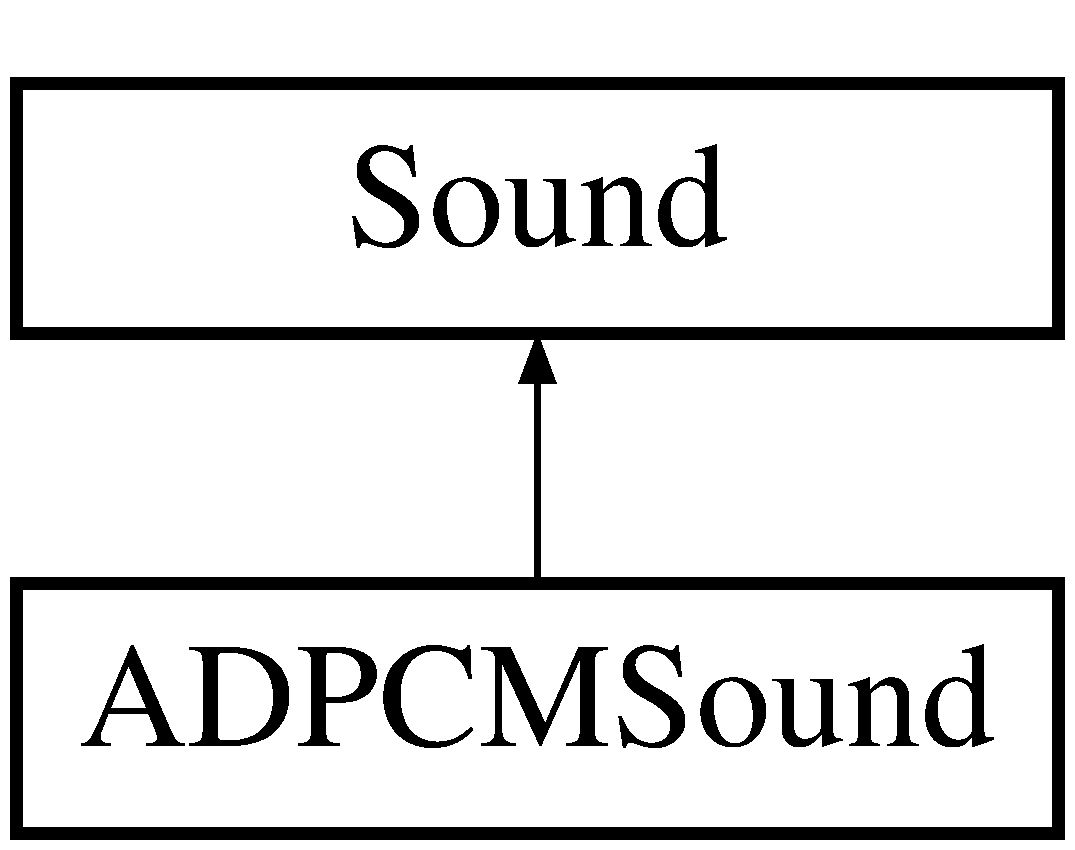
\includegraphics[height=2.000000cm]{class_a_d_p_c_m_sound}
\end{center}
\end{figure}
\subsection*{Public Member Functions}
\begin{DoxyCompactItemize}
\item 
\hyperlink{class_a_d_p_c_m_sound_a4213786af4c9c618d58955f8e83bfdca}{A\+D\+P\+C\+M\+Sound} (const unsigned char $\ast$data, int size)
\item 
virtual bool \hyperlink{class_a_d_p_c_m_sound_aa4bae7530240f47b76abef5dee718649}{fill\+Mono\+Buffer} (unsigned short $\ast$buffer, int size)
\item 
virtual bool \hyperlink{class_a_d_p_c_m_sound_a04e36f00fa43f9da21bc4bd97a2ddf44}{fill\+Stereo\+Buffer} (unsigned short $\ast$buffer, int length)
\item 
virtual void \hyperlink{class_a_d_p_c_m_sound_ac1c8d4b362dd7803087f82f3b26f6957}{rewind} ()
\end{DoxyCompactItemize}


\subsection{Detailed Description}
Class to play a buffer contatinig A\+D\+P\+CM compressed audio 

\subsection{Constructor \& Destructor Documentation}
\mbox{\Hypertarget{class_a_d_p_c_m_sound_a4213786af4c9c618d58955f8e83bfdca}\label{class_a_d_p_c_m_sound_a4213786af4c9c618d58955f8e83bfdca}} 
\index{A\+D\+P\+C\+M\+Sound@{A\+D\+P\+C\+M\+Sound}!A\+D\+P\+C\+M\+Sound@{A\+D\+P\+C\+M\+Sound}}
\index{A\+D\+P\+C\+M\+Sound@{A\+D\+P\+C\+M\+Sound}!A\+D\+P\+C\+M\+Sound@{A\+D\+P\+C\+M\+Sound}}
\subsubsection{\texorpdfstring{A\+D\+P\+C\+M\+Sound()}{ADPCMSound()}}
{\footnotesize\ttfamily A\+D\+P\+C\+M\+Sound\+::\+A\+D\+P\+C\+M\+Sound (\begin{DoxyParamCaption}\item[{const unsigned char $\ast$}]{data,  }\item[{int}]{size }\end{DoxyParamCaption})\hspace{0.3cm}{\ttfamily [inline]}}

Constructor 
\begin{DoxyParams}{Parameters}
{\em data} & A\+D\+P\+CM encoded data. Ownership of the buffer remains of the caller, which is responsible to make sure it remains valid for the entire lifetime of this class. This is not a problem in the expected use case of the buffer being const and static \\
\hline
{\em size} & size of data \\
\hline
\end{DoxyParams}


\subsection{Member Function Documentation}
\mbox{\Hypertarget{class_a_d_p_c_m_sound_aa4bae7530240f47b76abef5dee718649}\label{class_a_d_p_c_m_sound_aa4bae7530240f47b76abef5dee718649}} 
\index{A\+D\+P\+C\+M\+Sound@{A\+D\+P\+C\+M\+Sound}!fill\+Mono\+Buffer@{fill\+Mono\+Buffer}}
\index{fill\+Mono\+Buffer@{fill\+Mono\+Buffer}!A\+D\+P\+C\+M\+Sound@{A\+D\+P\+C\+M\+Sound}}
\subsubsection{\texorpdfstring{fill\+Mono\+Buffer()}{fillMonoBuffer()}}
{\footnotesize\ttfamily bool A\+D\+P\+C\+M\+Sound\+::fill\+Mono\+Buffer (\begin{DoxyParamCaption}\item[{unsigned short $\ast$}]{buffer,  }\item[{int}]{size }\end{DoxyParamCaption})\hspace{0.3cm}{\ttfamily [virtual]}}

Fill a buffer with audio samples 
\begin{DoxyParams}{Parameters}
{\em buffer} & a buffer where audio samples (16bit unsigned, 44100\+Hz) are to be stored. If there is not enough data to fill the entire buffer the remaining part must be filled with 0 \\
\hline
{\em length} & buffer length, must be divisible by two \\
\hline
\end{DoxyParams}
\begin{DoxyReturn}{Returns}
true if this is the last valif buffer (eof encountered) 
\end{DoxyReturn}


Implements \hyperlink{class_sound_aa0068675e952893d2fdfef2503bcbc81}{Sound}.

\mbox{\Hypertarget{class_a_d_p_c_m_sound_a04e36f00fa43f9da21bc4bd97a2ddf44}\label{class_a_d_p_c_m_sound_a04e36f00fa43f9da21bc4bd97a2ddf44}} 
\index{A\+D\+P\+C\+M\+Sound@{A\+D\+P\+C\+M\+Sound}!fill\+Stereo\+Buffer@{fill\+Stereo\+Buffer}}
\index{fill\+Stereo\+Buffer@{fill\+Stereo\+Buffer}!A\+D\+P\+C\+M\+Sound@{A\+D\+P\+C\+M\+Sound}}
\subsubsection{\texorpdfstring{fill\+Stereo\+Buffer()}{fillStereoBuffer()}}
{\footnotesize\ttfamily bool A\+D\+P\+C\+M\+Sound\+::fill\+Stereo\+Buffer (\begin{DoxyParamCaption}\item[{unsigned short $\ast$}]{buffer,  }\item[{int}]{length }\end{DoxyParamCaption})\hspace{0.3cm}{\ttfamily [virtual]}}

Fill a stereo buffer with audio samples 
\begin{DoxyParams}{Parameters}
{\em buffer} & a buffer where audio samples (16bit unsigned, 44100\+Hz) are to be stored. If there is not enough data to fill the entire buffer. The buffer format is alternating left-\/right samples, so buffer\mbox{[}0\mbox{]} is left buffer\mbox{[}1\mbox{]} is right, buffer\mbox{[}2\mbox{]} is again left... the remaining part must be filled with 0 \\
\hline
{\em length} & buffer length, must be divisible by four \\
\hline
\end{DoxyParams}
\begin{DoxyReturn}{Returns}
true if this is the last valif buffer (eof encountered) 
\end{DoxyReturn}


Implements \hyperlink{class_sound_ac514e0aa8963b40ddd328a9f79d0769b}{Sound}.

\mbox{\Hypertarget{class_a_d_p_c_m_sound_ac1c8d4b362dd7803087f82f3b26f6957}\label{class_a_d_p_c_m_sound_ac1c8d4b362dd7803087f82f3b26f6957}} 
\index{A\+D\+P\+C\+M\+Sound@{A\+D\+P\+C\+M\+Sound}!rewind@{rewind}}
\index{rewind@{rewind}!A\+D\+P\+C\+M\+Sound@{A\+D\+P\+C\+M\+Sound}}
\subsubsection{\texorpdfstring{rewind()}{rewind()}}
{\footnotesize\ttfamily void A\+D\+P\+C\+M\+Sound\+::rewind (\begin{DoxyParamCaption}{ }\end{DoxyParamCaption})\hspace{0.3cm}{\ttfamily [virtual]}}

Rewind the internal sound pointer so that succesive calls to fill\+Buffer() start brom the beginning of the sound. 

Implements \hyperlink{class_sound_a1870e3d50f0f58fc98fd966372ce42f1}{Sound}.



The documentation for this class was generated from the following files\+:\begin{DoxyCompactItemize}
\item 
\hyperlink{player_8h}{player.\+h}\item 
\hyperlink{player_8cpp}{player.\+cpp}\end{DoxyCompactItemize}

\hypertarget{class_player}{}\section{Player Class Reference}
\label{class_player}\index{Player@{Player}}


{\ttfamily \#include $<$player.\+h$>$}

\subsection*{Public Member Functions}
\begin{DoxyCompactItemize}
\item 
void \hyperlink{class_player_a895c8c46a9862e1c424720be3aa5e7d1}{play} (\hyperlink{class_sound}{Sound} \&sound)
\item 
bool \hyperlink{class_player_a06b5d53d568f357f77df80d0859fe8db}{is\+Playing} () const
\end{DoxyCompactItemize}
\subsection*{Static Public Member Functions}
\begin{DoxyCompactItemize}
\item 
static \hyperlink{class_player}{Player} \& \hyperlink{class_player_a2bf5cfb2a54c9fde1432fed9eb46fe49}{instance} ()
\end{DoxyCompactItemize}


\subsection{Detailed Description}
Class to play an audio file on the S\+T\+M32\textquotesingle{}s D\+AC 

\subsection{Member Function Documentation}
\mbox{\Hypertarget{class_player_a2bf5cfb2a54c9fde1432fed9eb46fe49}\label{class_player_a2bf5cfb2a54c9fde1432fed9eb46fe49}} 
\index{Player@{Player}!instance@{instance}}
\index{instance@{instance}!Player@{Player}}
\subsubsection{\texorpdfstring{instance()}{instance()}}
{\footnotesize\ttfamily \hyperlink{class_player}{Player} \& Player\+::instance (\begin{DoxyParamCaption}{ }\end{DoxyParamCaption})\hspace{0.3cm}{\ttfamily [static]}}

\begin{DoxyReturn}{Returns}
an instance of the player (singleton) 
\end{DoxyReturn}
\mbox{\Hypertarget{class_player_a06b5d53d568f357f77df80d0859fe8db}\label{class_player_a06b5d53d568f357f77df80d0859fe8db}} 
\index{Player@{Player}!is\+Playing@{is\+Playing}}
\index{is\+Playing@{is\+Playing}!Player@{Player}}
\subsubsection{\texorpdfstring{is\+Playing()}{isPlaying()}}
{\footnotesize\ttfamily bool Player\+::is\+Playing (\begin{DoxyParamCaption}{ }\end{DoxyParamCaption}) const}

\begin{DoxyReturn}{Returns}
true if the resource is busy 
\end{DoxyReturn}
\mbox{\Hypertarget{class_player_a895c8c46a9862e1c424720be3aa5e7d1}\label{class_player_a895c8c46a9862e1c424720be3aa5e7d1}} 
\index{Player@{Player}!play@{play}}
\index{play@{play}!Player@{Player}}
\subsubsection{\texorpdfstring{play()}{play()}}
{\footnotesize\ttfamily void Player\+::play (\begin{DoxyParamCaption}\item[{\hyperlink{class_sound}{Sound} \&}]{sound }\end{DoxyParamCaption})}

Play an audio file, returning after the file has coompleted playing 
\begin{DoxyParams}{Parameters}
{\em sound} & sound file to play \\
\hline
\end{DoxyParams}


The documentation for this class was generated from the following files\+:\begin{DoxyCompactItemize}
\item 
\hyperlink{player_8h}{player.\+h}\item 
\hyperlink{player_8cpp}{player.\+cpp}\end{DoxyCompactItemize}

\hypertarget{class_sound}{}\section{Sound Class Reference}
\label{class_sound}\index{Sound@{Sound}}


{\ttfamily \#include $<$player.\+h$>$}

Inheritance diagram for Sound\+:\begin{figure}[H]
\begin{center}
\leavevmode
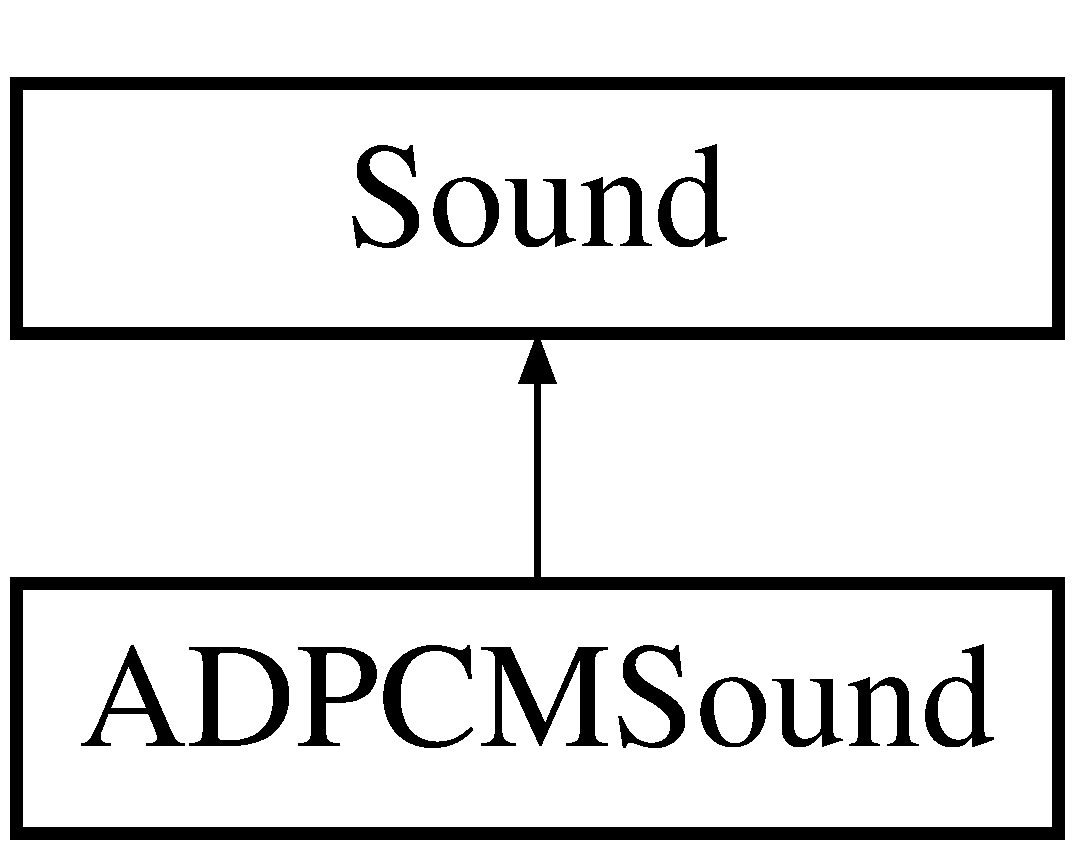
\includegraphics[height=2.000000cm]{class_sound}
\end{center}
\end{figure}
\subsection*{Public Member Functions}
\begin{DoxyCompactItemize}
\item 
virtual bool \hyperlink{class_sound_aa0068675e952893d2fdfef2503bcbc81}{fill\+Mono\+Buffer} (unsigned short $\ast$buffer, int length)=0
\item 
virtual bool \hyperlink{class_sound_ac514e0aa8963b40ddd328a9f79d0769b}{fill\+Stereo\+Buffer} (unsigned short $\ast$buffer, int length)=0
\item 
virtual void \hyperlink{class_sound_a1870e3d50f0f58fc98fd966372ce42f1}{rewind} ()=0
\item 
virtual \hyperlink{class_sound_a0907389078bf740be2a5763366ad3376}{$\sim$\+Sound} ()
\end{DoxyCompactItemize}


\subsection{Detailed Description}
Interface class from where all sound classes derive 

\subsection{Constructor \& Destructor Documentation}
\mbox{\Hypertarget{class_sound_a0907389078bf740be2a5763366ad3376}\label{class_sound_a0907389078bf740be2a5763366ad3376}} 
\index{Sound@{Sound}!````~Sound@{$\sim$\+Sound}}
\index{````~Sound@{$\sim$\+Sound}!Sound@{Sound}}
\subsubsection{\texorpdfstring{$\sim$\+Sound()}{~Sound()}}
{\footnotesize\ttfamily Sound\+::$\sim$\+Sound (\begin{DoxyParamCaption}{ }\end{DoxyParamCaption})\hspace{0.3cm}{\ttfamily [virtual]}}

Destructor 

\subsection{Member Function Documentation}
\mbox{\Hypertarget{class_sound_aa0068675e952893d2fdfef2503bcbc81}\label{class_sound_aa0068675e952893d2fdfef2503bcbc81}} 
\index{Sound@{Sound}!fill\+Mono\+Buffer@{fill\+Mono\+Buffer}}
\index{fill\+Mono\+Buffer@{fill\+Mono\+Buffer}!Sound@{Sound}}
\subsubsection{\texorpdfstring{fill\+Mono\+Buffer()}{fillMonoBuffer()}}
{\footnotesize\ttfamily virtual bool Sound\+::fill\+Mono\+Buffer (\begin{DoxyParamCaption}\item[{unsigned short $\ast$}]{buffer,  }\item[{int}]{length }\end{DoxyParamCaption})\hspace{0.3cm}{\ttfamily [pure virtual]}}

Fill a buffer with audio samples 
\begin{DoxyParams}{Parameters}
{\em buffer} & a buffer where audio samples (16bit unsigned, 44100\+Hz) are to be stored. If there is not enough data to fill the entire buffer the remaining part must be filled with 0 \\
\hline
{\em length} & buffer length, must be divisible by two \\
\hline
\end{DoxyParams}
\begin{DoxyReturn}{Returns}
true if this is the last valif buffer (eof encountered) 
\end{DoxyReturn}


Implemented in \hyperlink{class_a_d_p_c_m_sound_aa4bae7530240f47b76abef5dee718649}{A\+D\+P\+C\+M\+Sound}.

\mbox{\Hypertarget{class_sound_ac514e0aa8963b40ddd328a9f79d0769b}\label{class_sound_ac514e0aa8963b40ddd328a9f79d0769b}} 
\index{Sound@{Sound}!fill\+Stereo\+Buffer@{fill\+Stereo\+Buffer}}
\index{fill\+Stereo\+Buffer@{fill\+Stereo\+Buffer}!Sound@{Sound}}
\subsubsection{\texorpdfstring{fill\+Stereo\+Buffer()}{fillStereoBuffer()}}
{\footnotesize\ttfamily virtual bool Sound\+::fill\+Stereo\+Buffer (\begin{DoxyParamCaption}\item[{unsigned short $\ast$}]{buffer,  }\item[{int}]{length }\end{DoxyParamCaption})\hspace{0.3cm}{\ttfamily [pure virtual]}}

Fill a stereo buffer with audio samples 
\begin{DoxyParams}{Parameters}
{\em buffer} & a buffer where audio samples (16bit unsigned, 44100\+Hz) are to be stored. If there is not enough data to fill the entire buffer. The buffer format is alternating left-\/right samples, so buffer\mbox{[}0\mbox{]} is left buffer\mbox{[}1\mbox{]} is right, buffer\mbox{[}2\mbox{]} is again left... the remaining part must be filled with 0 \\
\hline
{\em length} & buffer length, must be divisible by four \\
\hline
\end{DoxyParams}
\begin{DoxyReturn}{Returns}
true if this is the last valif buffer (eof encountered) 
\end{DoxyReturn}


Implemented in \hyperlink{class_a_d_p_c_m_sound_a04e36f00fa43f9da21bc4bd97a2ddf44}{A\+D\+P\+C\+M\+Sound}.

\mbox{\Hypertarget{class_sound_a1870e3d50f0f58fc98fd966372ce42f1}\label{class_sound_a1870e3d50f0f58fc98fd966372ce42f1}} 
\index{Sound@{Sound}!rewind@{rewind}}
\index{rewind@{rewind}!Sound@{Sound}}
\subsubsection{\texorpdfstring{rewind()}{rewind()}}
{\footnotesize\ttfamily virtual void Sound\+::rewind (\begin{DoxyParamCaption}{ }\end{DoxyParamCaption})\hspace{0.3cm}{\ttfamily [pure virtual]}}

Rewind the internal sound pointer so that succesive calls to fill\+Buffer() start brom the beginning of the sound. 

Implemented in \hyperlink{class_a_d_p_c_m_sound_ac1c8d4b362dd7803087f82f3b26f6957}{A\+D\+P\+C\+M\+Sound}.



The documentation for this class was generated from the following files\+:\begin{DoxyCompactItemize}
\item 
\hyperlink{player_8h}{player.\+h}\item 
\hyperlink{player_8cpp}{player.\+cpp}\end{DoxyCompactItemize}

\chapter{File Documentation}
\hypertarget{adpcm_8c}{}\section{adpcm.\+c File Reference}
\label{adpcm_8c}\index{adpcm.\+c@{adpcm.\+c}}
{\ttfamily \#include \char`\"{}adpcm.\+h\char`\"{}}\newline
\subsection*{Functions}
\begin{DoxyCompactItemize}
\item 
uint8\+\_\+t \hyperlink{adpcm_8c_a8a44d2281064f8c97ecb4ccbec0d82eb}{A\+D\+P\+C\+M\+\_\+\+Encode} (int32\+\_\+t sample)
\begin{DoxyCompactList}\small\item\em A\+D\+P\+C\+M\+\_\+\+Encode. \end{DoxyCompactList}\item 
int16\+\_\+t \hyperlink{adpcm_8c_a7f7d41c4684389b2f0df1146cd86f15f}{A\+D\+P\+C\+M\+\_\+\+Decode} (uint8\+\_\+t code)
\begin{DoxyCompactList}\small\item\em A\+D\+P\+C\+M\+\_\+\+Decode. \end{DoxyCompactList}\end{DoxyCompactItemize}
\subsection*{Variables}
\begin{DoxyCompactItemize}
\item 
const uint16\+\_\+t \hyperlink{adpcm_8c_ae6f79ed9ab7b5abf97a1263c0faf2695}{Step\+Size\+Table} \mbox{[}89\mbox{]}
\item 
const int8\+\_\+t \hyperlink{adpcm_8c_aa7c5c6f7c5f5e97d6e7a0add664258f9}{Index\+Table} \mbox{[}16\mbox{]} =\{0xff,0xff,0xff,0xff,2,4,6,8,0xff,0xff,0xff,0xff,2,4,6,8\}
\end{DoxyCompactItemize}


\subsection{Function Documentation}
\mbox{\Hypertarget{adpcm_8c_a7f7d41c4684389b2f0df1146cd86f15f}\label{adpcm_8c_a7f7d41c4684389b2f0df1146cd86f15f}} 
\index{adpcm.\+c@{adpcm.\+c}!A\+D\+P\+C\+M\+\_\+\+Decode@{A\+D\+P\+C\+M\+\_\+\+Decode}}
\index{A\+D\+P\+C\+M\+\_\+\+Decode@{A\+D\+P\+C\+M\+\_\+\+Decode}!adpcm.\+c@{adpcm.\+c}}
\subsubsection{\texorpdfstring{A\+D\+P\+C\+M\+\_\+\+Decode()}{ADPCM\_Decode()}}
{\footnotesize\ttfamily int16\+\_\+t A\+D\+P\+C\+M\+\_\+\+Decode (\begin{DoxyParamCaption}\item[{uint8\+\_\+t}]{code }\end{DoxyParamCaption})}



A\+D\+P\+C\+M\+\_\+\+Decode. 


\begin{DoxyParams}{Parameters}
{\em code} & a byte containing a 4-\/bit A\+D\+P\+CM sample. \\
\hline
\end{DoxyParams}

\begin{DoxyRetVals}{Return values}
{\em } & 16-\/bit A\+D\+P\+CM sample \\
\hline
\end{DoxyRetVals}
\mbox{\Hypertarget{adpcm_8c_a8a44d2281064f8c97ecb4ccbec0d82eb}\label{adpcm_8c_a8a44d2281064f8c97ecb4ccbec0d82eb}} 
\index{adpcm.\+c@{adpcm.\+c}!A\+D\+P\+C\+M\+\_\+\+Encode@{A\+D\+P\+C\+M\+\_\+\+Encode}}
\index{A\+D\+P\+C\+M\+\_\+\+Encode@{A\+D\+P\+C\+M\+\_\+\+Encode}!adpcm.\+c@{adpcm.\+c}}
\subsubsection{\texorpdfstring{A\+D\+P\+C\+M\+\_\+\+Encode()}{ADPCM\_Encode()}}
{\footnotesize\ttfamily uint8\+\_\+t A\+D\+P\+C\+M\+\_\+\+Encode (\begin{DoxyParamCaption}\item[{int32\+\_\+t}]{sample }\end{DoxyParamCaption})}



A\+D\+P\+C\+M\+\_\+\+Encode. 


\begin{DoxyParams}{Parameters}
{\em sample} & a 16-\/bit P\+CM sample \\
\hline
\end{DoxyParams}

\begin{DoxyRetVals}{Return values}
{\em } & a 4-\/bit A\+D\+P\+CM sample \\
\hline
\end{DoxyRetVals}


\subsection{Variable Documentation}
\mbox{\Hypertarget{adpcm_8c_aa7c5c6f7c5f5e97d6e7a0add664258f9}\label{adpcm_8c_aa7c5c6f7c5f5e97d6e7a0add664258f9}} 
\index{adpcm.\+c@{adpcm.\+c}!Index\+Table@{Index\+Table}}
\index{Index\+Table@{Index\+Table}!adpcm.\+c@{adpcm.\+c}}
\subsubsection{\texorpdfstring{Index\+Table}{IndexTable}}
{\footnotesize\ttfamily const int8\+\_\+t Index\+Table\mbox{[}16\mbox{]} =\{0xff,0xff,0xff,0xff,2,4,6,8,0xff,0xff,0xff,0xff,2,4,6,8\}}

\mbox{\Hypertarget{adpcm_8c_ae6f79ed9ab7b5abf97a1263c0faf2695}\label{adpcm_8c_ae6f79ed9ab7b5abf97a1263c0faf2695}} 
\index{adpcm.\+c@{adpcm.\+c}!Step\+Size\+Table@{Step\+Size\+Table}}
\index{Step\+Size\+Table@{Step\+Size\+Table}!adpcm.\+c@{adpcm.\+c}}
\subsubsection{\texorpdfstring{Step\+Size\+Table}{StepSizeTable}}
{\footnotesize\ttfamily const uint16\+\_\+t Step\+Size\+Table\mbox{[}89\mbox{]}}

{\bfseries Initial value\+:}
\begin{DoxyCode}
=\{7,8,9,10,11,12,13,14,16,17,
                            19,21,23,25,28,31,34,37,41,45,
                            50,55,60,66,73,80,88,97,107,118,
                            130,143,157,173,190,209,230,253,279,307,
                            337,371,408,449,494,544,598,658,724,796,
                            876,963,1060,1166,1282,1411,1552,1707,1878,2066,
                            2272,2499,2749,3024,3327,3660,4026,4428,4871,5358,
                            5894,6484,7132,7845,8630,9493,10442,11487,12635,13899,
                            15289,16818,18500,20350,22385,24623,27086,29794,32767\}
\end{DoxyCode}

\hypertarget{adpcm_8d}{}\section{adpcm.\+d File Reference}
\label{adpcm_8d}\index{adpcm.\+d@{adpcm.\+d}}

\hypertarget{adpcm_8h}{}\section{adpcm.\+h File Reference}
\label{adpcm_8h}\index{adpcm.\+h@{adpcm.\+h}}
{\ttfamily \#include $<$stdint.\+h$>$}\newline
\subsection*{Functions}
\begin{DoxyCompactItemize}
\item 
uint8\+\_\+t \hyperlink{adpcm_8h_a8a44d2281064f8c97ecb4ccbec0d82eb}{A\+D\+P\+C\+M\+\_\+\+Encode} (int32\+\_\+t sample)
\begin{DoxyCompactList}\small\item\em A\+D\+P\+C\+M\+\_\+\+Encode. \end{DoxyCompactList}\item 
int16\+\_\+t \hyperlink{adpcm_8h_a7f7d41c4684389b2f0df1146cd86f15f}{A\+D\+P\+C\+M\+\_\+\+Decode} (uint8\+\_\+t code)
\begin{DoxyCompactList}\small\item\em A\+D\+P\+C\+M\+\_\+\+Decode. \end{DoxyCompactList}\end{DoxyCompactItemize}


\subsection{Function Documentation}
\mbox{\Hypertarget{adpcm_8h_a7f7d41c4684389b2f0df1146cd86f15f}\label{adpcm_8h_a7f7d41c4684389b2f0df1146cd86f15f}} 
\index{adpcm.\+h@{adpcm.\+h}!A\+D\+P\+C\+M\+\_\+\+Decode@{A\+D\+P\+C\+M\+\_\+\+Decode}}
\index{A\+D\+P\+C\+M\+\_\+\+Decode@{A\+D\+P\+C\+M\+\_\+\+Decode}!adpcm.\+h@{adpcm.\+h}}
\subsubsection{\texorpdfstring{A\+D\+P\+C\+M\+\_\+\+Decode()}{ADPCM\_Decode()}}
{\footnotesize\ttfamily int16\+\_\+t A\+D\+P\+C\+M\+\_\+\+Decode (\begin{DoxyParamCaption}\item[{uint8\+\_\+t}]{code }\end{DoxyParamCaption})}



A\+D\+P\+C\+M\+\_\+\+Decode. 


\begin{DoxyParams}{Parameters}
{\em code} & a byte containing a 4-\/bit A\+D\+P\+CM sample. \\
\hline
\end{DoxyParams}

\begin{DoxyRetVals}{Return values}
{\em } & 16-\/bit A\+D\+P\+CM sample \\
\hline
\end{DoxyRetVals}
\mbox{\Hypertarget{adpcm_8h_a8a44d2281064f8c97ecb4ccbec0d82eb}\label{adpcm_8h_a8a44d2281064f8c97ecb4ccbec0d82eb}} 
\index{adpcm.\+h@{adpcm.\+h}!A\+D\+P\+C\+M\+\_\+\+Encode@{A\+D\+P\+C\+M\+\_\+\+Encode}}
\index{A\+D\+P\+C\+M\+\_\+\+Encode@{A\+D\+P\+C\+M\+\_\+\+Encode}!adpcm.\+h@{adpcm.\+h}}
\subsubsection{\texorpdfstring{A\+D\+P\+C\+M\+\_\+\+Encode()}{ADPCM\_Encode()}}
{\footnotesize\ttfamily uint8\+\_\+t A\+D\+P\+C\+M\+\_\+\+Encode (\begin{DoxyParamCaption}\item[{int32\+\_\+t}]{sample }\end{DoxyParamCaption})}



A\+D\+P\+C\+M\+\_\+\+Encode. 


\begin{DoxyParams}{Parameters}
{\em sample} & a 16-\/bit P\+CM sample \\
\hline
\end{DoxyParams}

\begin{DoxyRetVals}{Return values}
{\em } & a 4-\/bit A\+D\+P\+CM sample \\
\hline
\end{DoxyRetVals}

\hypertarget{button_8cpp}{}\section{button.\+cpp File Reference}
\label{button_8cpp}\index{button.\+cpp@{button.\+cpp}}
{\ttfamily \#include \char`\"{}button.\+h\char`\"{}}\newline
{\ttfamily \#include $<$miosix.\+h$>$}\newline
{\ttfamily \#include $<$miosix/kernel/scheduler/scheduler.\+h$>$}\newline
{\ttfamily \#include $<$pthread.\+h$>$}\newline
\subsection*{Typedefs}
\begin{DoxyCompactItemize}
\item 
typedef Gpio$<$ G\+P\+I\+O\+A\+\_\+\+B\+A\+SE, 0 $>$ \hyperlink{button_8cpp_a9ec797ca62beef0ccb5999641933998a}{button}
\end{DoxyCompactItemize}
\subsection*{Functions}
\begin{DoxyCompactItemize}
\item 
void \hyperlink{button_8cpp_a39ff7bb2baa455c6e13bcdcbb47f5c18}{\+\_\+\+\_\+attribute\+\_\+\+\_\+} ((naked)) E\+X\+T\+I0\+\_\+\+I\+R\+Q\+Handler()
\item 
void \hyperlink{button_8cpp_a1b55748823e6e8521cdf9eff311d2213}{\+\_\+\+\_\+attribute\+\_\+\+\_\+} ((used)) E\+X\+T\+I0\+Handler\+Impl()
\item 
void \hyperlink{button_8cpp_af4bd66d08430d5410d40000c81ee8bac}{configure\+Button\+Interrupt} ()
\item 
void \hyperlink{button_8cpp_a906c879d4d5d9f61eb62e7c7d2845ffe}{wait\+For\+Button} ()
\end{DoxyCompactItemize}
\subsection*{Variables}
\begin{DoxyCompactItemize}
\item 
pthread\+\_\+mutex\+\_\+t \hyperlink{button_8cpp_a4acff8232e4aec9cd5c6dc200ac55ef3}{mutex}
\item 
bool \hyperlink{button_8cpp_ade51b3b01e72b5d342ac2e940e62b993}{action}
\end{DoxyCompactItemize}


\subsection{Detailed Description}
\begin{DoxyAuthor}{Author}
Federico Terraneo 

Simon Mastrodicasa 

Arne Vlietinck 
\end{DoxyAuthor}
\begin{DoxyVersion}{Version}
1.\+0 
\end{DoxyVersion}
\begin{DoxyDate}{Date}
22/12/2017 
\end{DoxyDate}


\subsection{Typedef Documentation}
\mbox{\Hypertarget{button_8cpp_a9ec797ca62beef0ccb5999641933998a}\label{button_8cpp_a9ec797ca62beef0ccb5999641933998a}} 
\index{button.\+cpp@{button.\+cpp}!button@{button}}
\index{button@{button}!button.\+cpp@{button.\+cpp}}
\subsubsection{\texorpdfstring{button}{button}}
{\footnotesize\ttfamily typedef Gpio$<$G\+P\+I\+O\+A\+\_\+\+B\+A\+SE,0$>$ \hyperlink{button_8cpp_a9ec797ca62beef0ccb5999641933998a}{button}}



\subsection{Function Documentation}
\mbox{\Hypertarget{button_8cpp_a39ff7bb2baa455c6e13bcdcbb47f5c18}\label{button_8cpp_a39ff7bb2baa455c6e13bcdcbb47f5c18}} 
\index{button.\+cpp@{button.\+cpp}!\+\_\+\+\_\+attribute\+\_\+\+\_\+@{\+\_\+\+\_\+attribute\+\_\+\+\_\+}}
\index{\+\_\+\+\_\+attribute\+\_\+\+\_\+@{\+\_\+\+\_\+attribute\+\_\+\+\_\+}!button.\+cpp@{button.\+cpp}}
\subsubsection{\texorpdfstring{\+\_\+\+\_\+attribute\+\_\+\+\_\+()}{\_\_attribute\_\_()}\hspace{0.1cm}{\footnotesize\ttfamily [1/2]}}
{\footnotesize\ttfamily void \+\_\+\+\_\+attribute\+\_\+\+\_\+ (\begin{DoxyParamCaption}\item[{(naked)}]{ }\end{DoxyParamCaption})}

\mbox{\Hypertarget{button_8cpp_a1b55748823e6e8521cdf9eff311d2213}\label{button_8cpp_a1b55748823e6e8521cdf9eff311d2213}} 
\index{button.\+cpp@{button.\+cpp}!\+\_\+\+\_\+attribute\+\_\+\+\_\+@{\+\_\+\+\_\+attribute\+\_\+\+\_\+}}
\index{\+\_\+\+\_\+attribute\+\_\+\+\_\+@{\+\_\+\+\_\+attribute\+\_\+\+\_\+}!button.\+cpp@{button.\+cpp}}
\subsubsection{\texorpdfstring{\+\_\+\+\_\+attribute\+\_\+\+\_\+()}{\_\_attribute\_\_()}\hspace{0.1cm}{\footnotesize\ttfamily [2/2]}}
{\footnotesize\ttfamily void \+\_\+\+\_\+attribute\+\_\+\+\_\+ (\begin{DoxyParamCaption}\item[{(used)}]{ }\end{DoxyParamCaption})}

\mbox{\Hypertarget{button_8cpp_af4bd66d08430d5410d40000c81ee8bac}\label{button_8cpp_af4bd66d08430d5410d40000c81ee8bac}} 
\index{button.\+cpp@{button.\+cpp}!configure\+Button\+Interrupt@{configure\+Button\+Interrupt}}
\index{configure\+Button\+Interrupt@{configure\+Button\+Interrupt}!button.\+cpp@{button.\+cpp}}
\subsubsection{\texorpdfstring{configure\+Button\+Interrupt()}{configureButtonInterrupt()}}
{\footnotesize\ttfamily void configure\+Button\+Interrupt (\begin{DoxyParamCaption}{ }\end{DoxyParamCaption})}

\mbox{\Hypertarget{button_8cpp_a906c879d4d5d9f61eb62e7c7d2845ffe}\label{button_8cpp_a906c879d4d5d9f61eb62e7c7d2845ffe}} 
\index{button.\+cpp@{button.\+cpp}!wait\+For\+Button@{wait\+For\+Button}}
\index{wait\+For\+Button@{wait\+For\+Button}!button.\+cpp@{button.\+cpp}}
\subsubsection{\texorpdfstring{wait\+For\+Button()}{waitForButton()}}
{\footnotesize\ttfamily void wait\+For\+Button (\begin{DoxyParamCaption}{ }\end{DoxyParamCaption})}



\subsection{Variable Documentation}
\mbox{\Hypertarget{button_8cpp_ade51b3b01e72b5d342ac2e940e62b993}\label{button_8cpp_ade51b3b01e72b5d342ac2e940e62b993}} 
\index{button.\+cpp@{button.\+cpp}!action@{action}}
\index{action@{action}!button.\+cpp@{button.\+cpp}}
\subsubsection{\texorpdfstring{action}{action}}
{\footnotesize\ttfamily bool action}

Boolean which representate the action of a player. When action is true, the player did an action. When action is false, the player didn\textquotesingle{}t do an action. \mbox{\Hypertarget{button_8cpp_a4acff8232e4aec9cd5c6dc200ac55ef3}\label{button_8cpp_a4acff8232e4aec9cd5c6dc200ac55ef3}} 
\index{button.\+cpp@{button.\+cpp}!mutex@{mutex}}
\index{mutex@{mutex}!button.\+cpp@{button.\+cpp}}
\subsubsection{\texorpdfstring{mutex}{mutex}}
{\footnotesize\ttfamily pthread\+\_\+mutex\+\_\+t mutex}

A pthread\+\_\+mutex\+\_\+t variable to prevent a race condition when changing action. 
\hypertarget{button_8d}{}\section{button.\+d File Reference}
\label{button_8d}\index{button.\+d@{button.\+d}}

\hypertarget{button_8h}{}\section{button.\+h File Reference}
\label{button_8h}\index{button.\+h@{button.\+h}}
\subsection*{Functions}
\begin{DoxyCompactItemize}
\item 
void \hyperlink{button_8h_af4bd66d08430d5410d40000c81ee8bac}{configure\+Button\+Interrupt} ()
\item 
void \hyperlink{button_8h_a906c879d4d5d9f61eb62e7c7d2845ffe}{wait\+For\+Button} ()
\end{DoxyCompactItemize}


\subsection{Detailed Description}
\begin{DoxyAuthor}{Author}
Federico Terraneo 

Simon Mastrodicasa 

Arne Vlietinck 
\end{DoxyAuthor}
\begin{DoxyVersion}{Version}
1.\+0 
\end{DoxyVersion}
\begin{DoxyDate}{Date}
30/12/2017 
\end{DoxyDate}


\subsection{Function Documentation}
\mbox{\Hypertarget{button_8h_af4bd66d08430d5410d40000c81ee8bac}\label{button_8h_af4bd66d08430d5410d40000c81ee8bac}} 
\index{button.\+h@{button.\+h}!configure\+Button\+Interrupt@{configure\+Button\+Interrupt}}
\index{configure\+Button\+Interrupt@{configure\+Button\+Interrupt}!button.\+h@{button.\+h}}
\subsubsection{\texorpdfstring{configure\+Button\+Interrupt()}{configureButtonInterrupt()}}
{\footnotesize\ttfamily void configure\+Button\+Interrupt (\begin{DoxyParamCaption}{ }\end{DoxyParamCaption})}

\mbox{\Hypertarget{button_8h_a906c879d4d5d9f61eb62e7c7d2845ffe}\label{button_8h_a906c879d4d5d9f61eb62e7c7d2845ffe}} 
\index{button.\+h@{button.\+h}!wait\+For\+Button@{wait\+For\+Button}}
\index{wait\+For\+Button@{wait\+For\+Button}!button.\+h@{button.\+h}}
\subsubsection{\texorpdfstring{wait\+For\+Button()}{waitForButton()}}
{\footnotesize\ttfamily void wait\+For\+Button (\begin{DoxyParamCaption}{ }\end{DoxyParamCaption})}


\hypertarget{buzzer_8h}{}\section{buzzer.\+h File Reference}
\label{buzzer_8h}\index{buzzer.\+h@{buzzer.\+h}}


The h-\/file for the buzzer sound. It contains the buzzer\+\_\+bin\mbox{[}\mbox{]}, which representates the char array for the buzzer sound to emphasize the fault of the player.  


\subsection*{Variables}
\begin{DoxyCompactItemize}
\item 
const unsigned char \hyperlink{buzzer_8h_a16fb99d8f19208fcdc658ed59f10ae1b}{buzzer\+\_\+bin} \mbox{[}$\,$\mbox{]}
\item 
const unsigned int \hyperlink{buzzer_8h_a9758d94719afe6199272d1c89870a1c4}{buzzer\+\_\+bin\+\_\+len} = 67392
\end{DoxyCompactItemize}


\subsection{Detailed Description}
The h-\/file for the buzzer sound. It contains the buzzer\+\_\+bin\mbox{[}\mbox{]}, which representates the char array for the buzzer sound to emphasize the fault of the player. 

\begin{DoxyAuthor}{Author}
Simon Mastrodicasa 

Arne Vlietinck 
\end{DoxyAuthor}
\begin{DoxyVersion}{Version}
1.\+0 
\end{DoxyVersion}
\begin{DoxyDate}{Date}
30/12/2017 
\end{DoxyDate}


\subsection{Variable Documentation}
\mbox{\Hypertarget{buzzer_8h_a16fb99d8f19208fcdc658ed59f10ae1b}\label{buzzer_8h_a16fb99d8f19208fcdc658ed59f10ae1b}} 
\index{buzzer.\+h@{buzzer.\+h}!buzzer\+\_\+bin@{buzzer\+\_\+bin}}
\index{buzzer\+\_\+bin@{buzzer\+\_\+bin}!buzzer.\+h@{buzzer.\+h}}
\subsubsection{\texorpdfstring{buzzer\+\_\+bin}{buzzer\_bin}}
{\footnotesize\ttfamily const unsigned char buzzer\+\_\+bin\mbox{[}$\,$\mbox{]}}

\mbox{\Hypertarget{buzzer_8h_a9758d94719afe6199272d1c89870a1c4}\label{buzzer_8h_a9758d94719afe6199272d1c89870a1c4}} 
\index{buzzer.\+h@{buzzer.\+h}!buzzer\+\_\+bin\+\_\+len@{buzzer\+\_\+bin\+\_\+len}}
\index{buzzer\+\_\+bin\+\_\+len@{buzzer\+\_\+bin\+\_\+len}!buzzer.\+h@{buzzer.\+h}}
\subsubsection{\texorpdfstring{buzzer\+\_\+bin\+\_\+len}{buzzer\_bin\_len}}
{\footnotesize\ttfamily const unsigned int buzzer\+\_\+bin\+\_\+len = 67392}


\hypertarget{convert_8cpp}{}\section{convert.\+cpp File Reference}
\label{convert_8cpp}\index{convert.\+cpp@{convert.\+cpp}}
{\ttfamily \#include $<$iostream$>$}\newline
{\ttfamily \#include $<$fstream$>$}\newline
{\ttfamily \#include $<$vector$>$}\newline
{\ttfamily \#include $<$cstdlib$>$}\newline
{\ttfamily \#include \char`\"{}adpcm.\+h\char`\"{}}\newline
\subsection*{Functions}
\begin{DoxyCompactItemize}
\item 
void \hyperlink{convert_8cpp_aa14887ab6108fdb498217f1625880d7b}{run} (const string \&s)
\item 
int \hyperlink{convert_8cpp_a0ddf1224851353fc92bfbff6f499fa97}{main} (int argc, char $\ast$argv\mbox{[}$\,$\mbox{]})
\end{DoxyCompactItemize}


\subsection{Function Documentation}
\mbox{\Hypertarget{convert_8cpp_a0ddf1224851353fc92bfbff6f499fa97}\label{convert_8cpp_a0ddf1224851353fc92bfbff6f499fa97}} 
\index{convert.\+cpp@{convert.\+cpp}!main@{main}}
\index{main@{main}!convert.\+cpp@{convert.\+cpp}}
\subsubsection{\texorpdfstring{main()}{main()}}
{\footnotesize\ttfamily int main (\begin{DoxyParamCaption}\item[{int}]{argc,  }\item[{char $\ast$}]{argv\mbox{[}$\,$\mbox{]} }\end{DoxyParamCaption})}

\mbox{\Hypertarget{convert_8cpp_aa14887ab6108fdb498217f1625880d7b}\label{convert_8cpp_aa14887ab6108fdb498217f1625880d7b}} 
\index{convert.\+cpp@{convert.\+cpp}!run@{run}}
\index{run@{run}!convert.\+cpp@{convert.\+cpp}}
\subsubsection{\texorpdfstring{run()}{run()}}
{\footnotesize\ttfamily void run (\begin{DoxyParamCaption}\item[{const string \&}]{s }\end{DoxyParamCaption})}


\hypertarget{game_8cpp}{}\section{game.\+cpp File Reference}
\label{game_8cpp}\index{game.\+cpp@{game.\+cpp}}


The cpp-\/file of the gameplay library.  


{\ttfamily \#include $<$miosix.\+h$>$}\newline
{\ttfamily \#include $<$pthread.\+h$>$}\newline
{\ttfamily \#include \char`\"{}game.\+h\char`\"{}}\newline
{\ttfamily \#include \char`\"{}led.\+h\char`\"{}}\newline
{\ttfamily \#include \char`\"{}player.\+h\char`\"{}}\newline
{\ttfamily \#include \char`\"{}buzzer.\+h\char`\"{}}\newline
{\ttfamily \#include \char`\"{}highscore.\+h\char`\"{}}\newline
\subsection*{Typedefs}
\begin{DoxyCompactItemize}
\item 
typedef Gpio$<$ G\+P\+I\+O\+A\+\_\+\+B\+A\+SE, 0 $>$ \hyperlink{game_8cpp_a9ec797ca62beef0ccb5999641933998a}{button}
\end{DoxyCompactItemize}
\subsection*{Functions}
\begin{DoxyCompactItemize}
\item 
bool \hyperlink{game_8cpp_a23d7d9d0b3ee3f4671ee1ec05b432f02}{should\+Blink\+Again} ()
\item 
void \hyperlink{game_8cpp_aa412aad3ea28593f7751a097bde6cf36}{buzzer\+Sound} ()
\item 
void \hyperlink{game_8cpp_ae626226c5eda23b723d67a2239b1dcf8}{highscore\+Sound} ()
\item 
void \hyperlink{game_8cpp_a026d019671eda0cfe729200fc24d23ba}{game\+Over} ()
\item 
int \hyperlink{game_8cpp_aa1607b7bd233c802d5d776c20b61ba9c}{game\+Play} (int current\+Led, bool clockwise)
\end{DoxyCompactItemize}
\subsection*{Variables}
\begin{DoxyCompactItemize}
\item 
bool \hyperlink{game_8cpp_ade51b3b01e72b5d342ac2e940e62b993}{action}
\item 
bool \hyperlink{game_8cpp_ad8f6d257142678d59a37901ccaff0438}{game}
\item 
bool \hyperlink{game_8cpp_ae7f4e2b17cc634cbab911507df1b899a}{interaction}
\item 
int \hyperlink{game_8cpp_a016a5d341f375d13639c75bf5987fb23}{difficulty}
\item 
int \hyperlink{game_8cpp_acf4d33ee4cff36f69b924471174dcb11}{level}
\item 
int \hyperlink{game_8cpp_ae5e9542e61196e233d289084760e4ab1}{highscore}
\item 
pthread\+\_\+mutex\+\_\+t \hyperlink{game_8cpp_a4acff8232e4aec9cd5c6dc200ac55ef3}{mutex}
\end{DoxyCompactItemize}


\subsection{Detailed Description}
The cpp-\/file of the gameplay library. 

\begin{DoxyAuthor}{Author}
Simon Mastrodicasa 

Arne Vlietinck 
\end{DoxyAuthor}
\begin{DoxyVersion}{Version}
1.\+0 
\end{DoxyVersion}
\begin{DoxyDate}{Date}
30/12/2017 
\end{DoxyDate}


\subsection{Typedef Documentation}
\mbox{\Hypertarget{game_8cpp_a9ec797ca62beef0ccb5999641933998a}\label{game_8cpp_a9ec797ca62beef0ccb5999641933998a}} 
\index{game.\+cpp@{game.\+cpp}!button@{button}}
\index{button@{button}!game.\+cpp@{game.\+cpp}}
\subsubsection{\texorpdfstring{button}{button}}
{\footnotesize\ttfamily typedef Gpio$<$G\+P\+I\+O\+A\+\_\+\+B\+A\+SE,0$>$ \hyperlink{button_8cpp_a9ec797ca62beef0ccb5999641933998a}{button}}



\subsection{Function Documentation}
\mbox{\Hypertarget{game_8cpp_aa412aad3ea28593f7751a097bde6cf36}\label{game_8cpp_aa412aad3ea28593f7751a097bde6cf36}} 
\index{game.\+cpp@{game.\+cpp}!buzzer\+Sound@{buzzer\+Sound}}
\index{buzzer\+Sound@{buzzer\+Sound}!game.\+cpp@{game.\+cpp}}
\subsubsection{\texorpdfstring{buzzer\+Sound()}{buzzerSound()}}
{\footnotesize\ttfamily void buzzer\+Sound (\begin{DoxyParamCaption}{ }\end{DoxyParamCaption})}

Function which plays the buzzer sound. \mbox{\Hypertarget{game_8cpp_a026d019671eda0cfe729200fc24d23ba}\label{game_8cpp_a026d019671eda0cfe729200fc24d23ba}} 
\index{game.\+cpp@{game.\+cpp}!game\+Over@{game\+Over}}
\index{game\+Over@{game\+Over}!game.\+cpp@{game.\+cpp}}
\subsubsection{\texorpdfstring{game\+Over()}{gameOver()}}
{\footnotesize\ttfamily void game\+Over (\begin{DoxyParamCaption}{ }\end{DoxyParamCaption})}

Function which does the game\+Over ritual.

\begin{DoxyPostcond}{Postcondition}
If and only if (level$>$highscore), the high score sound is played. 

If and only if (level$>$highscore), highscore is set to level. 

If (level$<$=highscore), the buzzer sound is played. 

The game\+Over blinking ritual is played. 

Game is set to G\+A\+M\+E\+O\+V\+ER. 
\end{DoxyPostcond}
\begin{DoxySeeAlso}{See also}
\hyperlink{game_8h_aa412aad3ea28593f7751a097bde6cf36}{buzzer\+Sound()} 

\hyperlink{game_8h_ae626226c5eda23b723d67a2239b1dcf8}{highscore\+Sound()} 

\hyperlink{led_8cpp_a31f84df1fa36897540314bb58287137a}{on\+Off\+Blinking()} 
\end{DoxySeeAlso}
\mbox{\Hypertarget{game_8cpp_aa1607b7bd233c802d5d776c20b61ba9c}\label{game_8cpp_aa1607b7bd233c802d5d776c20b61ba9c}} 
\index{game.\+cpp@{game.\+cpp}!game\+Play@{game\+Play}}
\index{game\+Play@{game\+Play}!game.\+cpp@{game.\+cpp}}
\subsubsection{\texorpdfstring{game\+Play()}{gamePlay()}}
{\footnotesize\ttfamily int game\+Play (\begin{DoxyParamCaption}\item[{int}]{current\+Led,  }\item[{bool}]{clockwise }\end{DoxyParamCaption})}

Function which takes care of the gameplay. It checks the several possible conditions and increment or decrement the several game parameters. When the player did a wrong interaction the gameover ritual is started.


\begin{DoxyParams}{Parameters}
{\em int} & currentled -\/ The number of the current L\+ED. \\
\hline
{\em bool} & clockwise -\/ Represents the order of blinking the L\+ED\textquotesingle{}s. \\
\hline
\end{DoxyParams}
\begin{DoxyPostcond}{Postcondition}
If and only if (interaction==false \&\& \hyperlink{game_8h_a23d7d9d0b3ee3f4671ee1ec05b432f02}{should\+Blink\+Again()}==true), interaction is set true. 

If (interaction==true \&\& action==false), \hyperlink{game_8h_a026d019671eda0cfe729200fc24d23ba}{game\+Over()} is excecuted. 

If (interaction==false \&\& action==true), \hyperlink{game_8h_a026d019671eda0cfe729200fc24d23ba}{game\+Over()} is excecuted. 

If and only if (interaction==true \&\& action==true), interaction is set false. 

If and only if (interaction==true \&\& action==true), action is set false. 

If and only if (interaction==true \&\& action==true), difficulty is incremented by one. 

If and only if (interaction==true \&\& action==true), level is incremented by one. 

If and only if (clockwise==true), current\+Led is incremented by one. 

If and only if (clockwise!=false), current\+Led is decremented by one. 

If and only if (current\+Led$>$R\+ED), current\+Led is set to the smallest L\+ED (B\+L\+UE). 

If and only if (current\+Led$<$B\+L\+UE), current\+Led is set to the biggest L\+ED (R\+ED). 
\end{DoxyPostcond}
\begin{DoxyReturn}{Returns}
int current\+Led -\/ The number of the current L\+ED. 
\end{DoxyReturn}
\begin{DoxySeeAlso}{See also}
\hyperlink{game_8h_a026d019671eda0cfe729200fc24d23ba}{game\+Over()} 

\hyperlink{game_8h_a23d7d9d0b3ee3f4671ee1ec05b432f02}{should\+Blink\+Again()}; 
\end{DoxySeeAlso}
\mbox{\Hypertarget{game_8cpp_ae626226c5eda23b723d67a2239b1dcf8}\label{game_8cpp_ae626226c5eda23b723d67a2239b1dcf8}} 
\index{game.\+cpp@{game.\+cpp}!highscore\+Sound@{highscore\+Sound}}
\index{highscore\+Sound@{highscore\+Sound}!game.\+cpp@{game.\+cpp}}
\subsubsection{\texorpdfstring{highscore\+Sound()}{highscoreSound()}}
{\footnotesize\ttfamily void highscore\+Sound (\begin{DoxyParamCaption}{ }\end{DoxyParamCaption})}

Function which plays the high score sound. \mbox{\Hypertarget{game_8cpp_a23d7d9d0b3ee3f4671ee1ec05b432f02}\label{game_8cpp_a23d7d9d0b3ee3f4671ee1ec05b432f02}} 
\index{game.\+cpp@{game.\+cpp}!should\+Blink\+Again@{should\+Blink\+Again}}
\index{should\+Blink\+Again@{should\+Blink\+Again}!game.\+cpp@{game.\+cpp}}
\subsubsection{\texorpdfstring{should\+Blink\+Again()}{shouldBlinkAgain()}}
{\footnotesize\ttfamily bool should\+Blink\+Again (\begin{DoxyParamCaption}{ }\end{DoxyParamCaption})}

Function which calculate if the L\+ED should blink for a second time.

\begin{DoxyReturn}{Returns}
Returns a random boolean which tells if the L\+ED should blink again. 
\end{DoxyReturn}
\begin{DoxyNote}{Note}
The boolean is in 30\% of the situations true and in the other 70\% false. 
\end{DoxyNote}


\subsection{Variable Documentation}
\mbox{\Hypertarget{game_8cpp_ade51b3b01e72b5d342ac2e940e62b993}\label{game_8cpp_ade51b3b01e72b5d342ac2e940e62b993}} 
\index{game.\+cpp@{game.\+cpp}!action@{action}}
\index{action@{action}!game.\+cpp@{game.\+cpp}}
\subsubsection{\texorpdfstring{action}{action}}
{\footnotesize\ttfamily bool action}

Boolean which represents the action of a player. If (action==true), the player did an action. Elseif (action==false), the player didn\textquotesingle{}t do an action. \mbox{\Hypertarget{game_8cpp_a016a5d341f375d13639c75bf5987fb23}\label{game_8cpp_a016a5d341f375d13639c75bf5987fb23}} 
\index{game.\+cpp@{game.\+cpp}!difficulty@{difficulty}}
\index{difficulty@{difficulty}!game.\+cpp@{game.\+cpp}}
\subsubsection{\texorpdfstring{difficulty}{difficulty}}
{\footnotesize\ttfamily int difficulty}

Integer which represents the difficulty level of the game. Higher integer means higher degree of difficulty. It affects the time between the blinking L\+ED\textquotesingle{}s. \mbox{\Hypertarget{game_8cpp_ad8f6d257142678d59a37901ccaff0438}\label{game_8cpp_ad8f6d257142678d59a37901ccaff0438}} 
\index{game.\+cpp@{game.\+cpp}!game@{game}}
\index{game@{game}!game.\+cpp@{game.\+cpp}}
\subsubsection{\texorpdfstring{game}{game}}
{\footnotesize\ttfamily bool game}

Boolean which represents the state of the game. If (game==1), the current game is finished. Elseif (game==0), the current game is still running. \mbox{\Hypertarget{game_8cpp_ae5e9542e61196e233d289084760e4ab1}\label{game_8cpp_ae5e9542e61196e233d289084760e4ab1}} 
\index{game.\+cpp@{game.\+cpp}!highscore@{highscore}}
\index{highscore@{highscore}!game.\+cpp@{game.\+cpp}}
\subsubsection{\texorpdfstring{highscore}{highscore}}
{\footnotesize\ttfamily int highscore}

Integer which represents the current high score of the game. \mbox{\Hypertarget{game_8cpp_ae7f4e2b17cc634cbab911507df1b899a}\label{game_8cpp_ae7f4e2b17cc634cbab911507df1b899a}} 
\index{game.\+cpp@{game.\+cpp}!interaction@{interaction}}
\index{interaction@{interaction}!game.\+cpp@{game.\+cpp}}
\subsubsection{\texorpdfstring{interaction}{interaction}}
{\footnotesize\ttfamily bool interaction}

Boolean which represents the need of a players\textquotesingle{} interaction. When interaction is true, the player must do something (e.\+g. press the user button) to avoid a game over. \mbox{\Hypertarget{game_8cpp_acf4d33ee4cff36f69b924471174dcb11}\label{game_8cpp_acf4d33ee4cff36f69b924471174dcb11}} 
\index{game.\+cpp@{game.\+cpp}!level@{level}}
\index{level@{level}!game.\+cpp@{game.\+cpp}}
\subsubsection{\texorpdfstring{level}{level}}
{\footnotesize\ttfamily int level}

Integer which represents the level of the game. \mbox{\Hypertarget{game_8cpp_a4acff8232e4aec9cd5c6dc200ac55ef3}\label{game_8cpp_a4acff8232e4aec9cd5c6dc200ac55ef3}} 
\index{game.\+cpp@{game.\+cpp}!mutex@{mutex}}
\index{mutex@{mutex}!game.\+cpp@{game.\+cpp}}
\subsubsection{\texorpdfstring{mutex}{mutex}}
{\footnotesize\ttfamily pthread\+\_\+mutex\+\_\+t mutex}

A pthread\+\_\+mutex\+\_\+t variable to prevent a race condition when changing action. 
\hypertarget{game_8d}{}\section{game.\+d File Reference}
\label{game_8d}\index{game.\+d@{game.\+d}}

\hypertarget{game_8h}{}\section{game.\+h File Reference}
\label{game_8h}\index{game.\+h@{game.\+h}}


The h-\/file of the gameplay library.  


\subsection*{Macros}
\begin{DoxyCompactItemize}
\item 
\#define \hyperlink{game_8h_aa71f1218eb9aadc17420151c26ac8f9c}{G\+A\+M\+E\+O\+V\+ER}~1
\end{DoxyCompactItemize}
\subsection*{Functions}
\begin{DoxyCompactItemize}
\item 
bool \hyperlink{game_8h_a23d7d9d0b3ee3f4671ee1ec05b432f02}{should\+Blink\+Again} ()
\item 
void \hyperlink{game_8h_aa412aad3ea28593f7751a097bde6cf36}{buzzer\+Sound} ()
\item 
void \hyperlink{game_8h_ae626226c5eda23b723d67a2239b1dcf8}{highscore\+Sound} ()
\item 
void \hyperlink{game_8h_a026d019671eda0cfe729200fc24d23ba}{game\+Over} ()
\item 
int \hyperlink{game_8h_aa1607b7bd233c802d5d776c20b61ba9c}{game\+Play} (int current\+Led, bool clockwise)
\end{DoxyCompactItemize}


\subsection{Detailed Description}
The h-\/file of the gameplay library. 

\begin{DoxyAuthor}{Author}
Simon Mastrodicasa 

Arne Vlietinck 
\end{DoxyAuthor}
\begin{DoxyVersion}{Version}
1.\+0 
\end{DoxyVersion}
\begin{DoxyDate}{Date}
22/12/2017 
\end{DoxyDate}


\subsection{Macro Definition Documentation}
\mbox{\Hypertarget{game_8h_aa71f1218eb9aadc17420151c26ac8f9c}\label{game_8h_aa71f1218eb9aadc17420151c26ac8f9c}} 
\index{game.\+h@{game.\+h}!G\+A\+M\+E\+O\+V\+ER@{G\+A\+M\+E\+O\+V\+ER}}
\index{G\+A\+M\+E\+O\+V\+ER@{G\+A\+M\+E\+O\+V\+ER}!game.\+h@{game.\+h}}
\subsubsection{\texorpdfstring{G\+A\+M\+E\+O\+V\+ER}{GAMEOVER}}
{\footnotesize\ttfamily \#define G\+A\+M\+E\+O\+V\+ER~1}



\subsection{Function Documentation}
\mbox{\Hypertarget{game_8h_aa412aad3ea28593f7751a097bde6cf36}\label{game_8h_aa412aad3ea28593f7751a097bde6cf36}} 
\index{game.\+h@{game.\+h}!buzzer\+Sound@{buzzer\+Sound}}
\index{buzzer\+Sound@{buzzer\+Sound}!game.\+h@{game.\+h}}
\subsubsection{\texorpdfstring{buzzer\+Sound()}{buzzerSound()}}
{\footnotesize\ttfamily void buzzer\+Sound (\begin{DoxyParamCaption}{ }\end{DoxyParamCaption})}

Function which plays the buzzer sound. \mbox{\Hypertarget{game_8h_a026d019671eda0cfe729200fc24d23ba}\label{game_8h_a026d019671eda0cfe729200fc24d23ba}} 
\index{game.\+h@{game.\+h}!game\+Over@{game\+Over}}
\index{game\+Over@{game\+Over}!game.\+h@{game.\+h}}
\subsubsection{\texorpdfstring{game\+Over()}{gameOver()}}
{\footnotesize\ttfamily void game\+Over (\begin{DoxyParamCaption}{ }\end{DoxyParamCaption})}

Function which does the game\+Over ritual.

\begin{DoxyPostcond}{Postcondition}
If and only if (level$>$highscore), the highscore sound is played. 

If and only if (level$>$highscore), highscore is set to level. 

If (level$<$=highscore), the buzzer sound is played. 

The game\+Over blinking ritual is played. 

Game is set to G\+A\+M\+E\+O\+V\+ER. 
\end{DoxyPostcond}
\begin{DoxySeeAlso}{See also}
\hyperlink{game_8h_aa412aad3ea28593f7751a097bde6cf36}{buzzer\+Sound()} 

\hyperlink{game_8h_ae626226c5eda23b723d67a2239b1dcf8}{highscore\+Sound()} 

\hyperlink{led_8cpp_a31f84df1fa36897540314bb58287137a}{on\+Off\+Blinking()} 
\end{DoxySeeAlso}
\mbox{\Hypertarget{game_8h_aa1607b7bd233c802d5d776c20b61ba9c}\label{game_8h_aa1607b7bd233c802d5d776c20b61ba9c}} 
\index{game.\+h@{game.\+h}!game\+Play@{game\+Play}}
\index{game\+Play@{game\+Play}!game.\+h@{game.\+h}}
\subsubsection{\texorpdfstring{game\+Play()}{gamePlay()}}
{\footnotesize\ttfamily int game\+Play (\begin{DoxyParamCaption}\item[{int}]{current\+Led,  }\item[{bool}]{clockwise }\end{DoxyParamCaption})}

Function which takes care of the gameplay. It checks the several possible conditions and increment or decrement the several game parameters. When the player did a wrong interaction the gameover ritual is started.


\begin{DoxyParams}{Parameters}
{\em int} & currentled -\/ The number of the current L\+ED. \\
\hline
{\em bool} & clockwise -\/ Represents the order of blinking the L\+ED\textquotesingle{}s. \\
\hline
\end{DoxyParams}
\begin{DoxyPostcond}{Postcondition}
If and only if (interaction==false \&\& \hyperlink{game_8h_a23d7d9d0b3ee3f4671ee1ec05b432f02}{should\+Blink\+Again()}==true), interaction is set true. 

If (interaction==true \&\& action==false), \hyperlink{game_8h_a026d019671eda0cfe729200fc24d23ba}{game\+Over()} is excecuted. 

If (interaction==false \&\& action==true), \hyperlink{game_8h_a026d019671eda0cfe729200fc24d23ba}{game\+Over()} is excecuted. 

If and only if (interaction==true \&\& action==true), interaction is set false. 

If and only if (interaction==true \&\& action==true), action is set false. 

If and only if (interaction==true \&\& action==true), difficulty is incremented by one. 

If and only if (interaction==true \&\& action==true), level is incremented by one. 

If and only if (clockwise==true), current\+Led is incremented by one. 

If and only if (clockwise!=false), current\+Led is decremented by one. 

If and only if (current\+Led$>$R\+ED), current\+Led is set to the smallest L\+ED (B\+L\+UE). 

If and only if (current\+Led$<$B\+L\+UE), current\+Led is set to the biggest L\+ED (R\+ED). 
\end{DoxyPostcond}
\begin{DoxyReturn}{Returns}
int current\+Led -\/ The number of the current L\+ED. 
\end{DoxyReturn}
\begin{DoxySeeAlso}{See also}
\hyperlink{game_8h_a026d019671eda0cfe729200fc24d23ba}{game\+Over()} 

\hyperlink{game_8h_a23d7d9d0b3ee3f4671ee1ec05b432f02}{should\+Blink\+Again()}; 
\end{DoxySeeAlso}
\mbox{\Hypertarget{game_8h_ae626226c5eda23b723d67a2239b1dcf8}\label{game_8h_ae626226c5eda23b723d67a2239b1dcf8}} 
\index{game.\+h@{game.\+h}!highscore\+Sound@{highscore\+Sound}}
\index{highscore\+Sound@{highscore\+Sound}!game.\+h@{game.\+h}}
\subsubsection{\texorpdfstring{highscore\+Sound()}{highscoreSound()}}
{\footnotesize\ttfamily void highscore\+Sound (\begin{DoxyParamCaption}{ }\end{DoxyParamCaption})}

Function which plays the highscore sound. \mbox{\Hypertarget{game_8h_a23d7d9d0b3ee3f4671ee1ec05b432f02}\label{game_8h_a23d7d9d0b3ee3f4671ee1ec05b432f02}} 
\index{game.\+h@{game.\+h}!should\+Blink\+Again@{should\+Blink\+Again}}
\index{should\+Blink\+Again@{should\+Blink\+Again}!game.\+h@{game.\+h}}
\subsubsection{\texorpdfstring{should\+Blink\+Again()}{shouldBlinkAgain()}}
{\footnotesize\ttfamily bool should\+Blink\+Again (\begin{DoxyParamCaption}{ }\end{DoxyParamCaption})}

Function which calculate if the L\+ED should blink for a second time.

\begin{DoxyReturn}{Returns}
Returns a random boolean which tells if the L\+ED should blink again. 
\end{DoxyReturn}
\begin{DoxyNote}{Note}
The boolean is in 30\% of the situations true and in the other 70\% false. 
\end{DoxyNote}

\hypertarget{highscore_8h}{}\section{highscore.\+h File Reference}
\label{highscore_8h}\index{highscore.\+h@{highscore.\+h}}


The h-\/file for the high score sound. It contains the highscore\+\_\+bin\mbox{[}\mbox{]}, which representates the char array for the high score sound to emphasize a new high score of the player.  


\subsection*{Variables}
\begin{DoxyCompactItemize}
\item 
const unsigned char \hyperlink{highscore_8h_a6be4aeb462e121d560da46f01f6dfd78}{highscore\+\_\+bin} \mbox{[}$\,$\mbox{]}
\item 
const unsigned int \hyperlink{highscore_8h_ae4a5ca9c808f29ac778d6510c95cbdaf}{highscore\+\_\+bin\+\_\+len} = 136366
\end{DoxyCompactItemize}


\subsection{Detailed Description}
The h-\/file for the high score sound. It contains the highscore\+\_\+bin\mbox{[}\mbox{]}, which representates the char array for the high score sound to emphasize a new high score of the player. 

\begin{DoxyAuthor}{Author}
Simon Mastrodicasa 

Arne Vlietinck 
\end{DoxyAuthor}
\begin{DoxyVersion}{Version}
1.\+0 
\end{DoxyVersion}
\begin{DoxyDate}{Date}
30/12/2017 
\end{DoxyDate}


\subsection{Variable Documentation}
\mbox{\Hypertarget{highscore_8h_a6be4aeb462e121d560da46f01f6dfd78}\label{highscore_8h_a6be4aeb462e121d560da46f01f6dfd78}} 
\index{highscore.\+h@{highscore.\+h}!highscore\+\_\+bin@{highscore\+\_\+bin}}
\index{highscore\+\_\+bin@{highscore\+\_\+bin}!highscore.\+h@{highscore.\+h}}
\subsubsection{\texorpdfstring{highscore\+\_\+bin}{highscore\_bin}}
{\footnotesize\ttfamily const unsigned char highscore\+\_\+bin\mbox{[}$\,$\mbox{]}}

\mbox{\Hypertarget{highscore_8h_ae4a5ca9c808f29ac778d6510c95cbdaf}\label{highscore_8h_ae4a5ca9c808f29ac778d6510c95cbdaf}} 
\index{highscore.\+h@{highscore.\+h}!highscore\+\_\+bin\+\_\+len@{highscore\+\_\+bin\+\_\+len}}
\index{highscore\+\_\+bin\+\_\+len@{highscore\+\_\+bin\+\_\+len}!highscore.\+h@{highscore.\+h}}
\subsubsection{\texorpdfstring{highscore\+\_\+bin\+\_\+len}{highscore\_bin\_len}}
{\footnotesize\ttfamily const unsigned int highscore\+\_\+bin\+\_\+len = 136366}


\hypertarget{led_8cpp}{}\section{led.\+cpp File Reference}
\label{led_8cpp}\index{led.\+cpp@{led.\+cpp}}
{\ttfamily \#include $<$miosix.\+h$>$}\newline
{\ttfamily \#include \char`\"{}led.\+h\char`\"{}}\newline
{\ttfamily \#include \char`\"{}game.\+h\char`\"{}}\newline
\subsection*{Typedefs}
\begin{DoxyCompactItemize}
\item 
typedef Gpio$<$ G\+P\+I\+O\+D\+\_\+\+B\+A\+SE, 12 $>$ \hyperlink{led_8cpp_a6745b7d47554307c3074e20c768fdbf0}{green\+Led}
\item 
typedef Gpio$<$ G\+P\+I\+O\+D\+\_\+\+B\+A\+SE, 13 $>$ \hyperlink{led_8cpp_a6945ae649b3a1e66a8b305907ae3d5cc}{orange\+Led}
\item 
typedef Gpio$<$ G\+P\+I\+O\+D\+\_\+\+B\+A\+SE, 14 $>$ \hyperlink{led_8cpp_ac320b3569ef011b726ff654b895ac0da}{red\+Led}
\item 
typedef Gpio$<$ G\+P\+I\+O\+D\+\_\+\+B\+A\+SE, 15 $>$ \hyperlink{led_8cpp_abf9b2336e2a6311d03233684fbbfb4a0}{blue\+Led}
\end{DoxyCompactItemize}
\subsection*{Functions}
\begin{DoxyCompactItemize}
\item 
void \hyperlink{led_8cpp_ad7bef4224d21ecc2b1c163529be7e406}{init\+Leds} ()
\item 
int \hyperlink{led_8cpp_a26142695353c128f29762dd3b6a3f54b}{calculate\+Sleep\+Time} (int \hyperlink{main_8cpp_a016a5d341f375d13639c75bf5987fb23}{difficulty})
\item 
void \hyperlink{led_8cpp_a6c6d18df77cca231909b6b527e686eff}{blinking\+Game} ()
\item 
void \hyperlink{led_8cpp_a39576974b484c2b69eeea478fc858e63}{turn\+All\+On} ()
\item 
void \hyperlink{led_8cpp_a84f6740c06243b975019d0b1b1a633d2}{turn\+All\+Off} ()
\item 
void \hyperlink{led_8cpp_a26db556312ad51df071dcff1e7943182}{game\+Over\+Blinking} ()
\end{DoxyCompactItemize}
\subsection*{Variables}
\begin{DoxyCompactItemize}
\item 
bool \hyperlink{led_8cpp_ad8f6d257142678d59a37901ccaff0438}{game}
\item 
int \hyperlink{led_8cpp_a016a5d341f375d13639c75bf5987fb23}{difficulty}
\end{DoxyCompactItemize}


\subsection{Detailed Description}
\begin{DoxyAuthor}{Author}
Simon Mastrodicasa 

Arne Vlietinck 
\end{DoxyAuthor}
\begin{DoxyVersion}{Version}
1.\+0 
\end{DoxyVersion}
\begin{DoxyDate}{Date}
22/12/2017 
\end{DoxyDate}


\subsection{Typedef Documentation}
\mbox{\Hypertarget{led_8cpp_abf9b2336e2a6311d03233684fbbfb4a0}\label{led_8cpp_abf9b2336e2a6311d03233684fbbfb4a0}} 
\index{led.\+cpp@{led.\+cpp}!blue\+Led@{blue\+Led}}
\index{blue\+Led@{blue\+Led}!led.\+cpp@{led.\+cpp}}
\subsubsection{\texorpdfstring{blue\+Led}{blueLed}}
{\footnotesize\ttfamily typedef Gpio$<$G\+P\+I\+O\+D\+\_\+\+B\+A\+SE,15$>$ \hyperlink{led_8cpp_abf9b2336e2a6311d03233684fbbfb4a0}{blue\+Led}}

\mbox{\Hypertarget{led_8cpp_a6745b7d47554307c3074e20c768fdbf0}\label{led_8cpp_a6745b7d47554307c3074e20c768fdbf0}} 
\index{led.\+cpp@{led.\+cpp}!green\+Led@{green\+Led}}
\index{green\+Led@{green\+Led}!led.\+cpp@{led.\+cpp}}
\subsubsection{\texorpdfstring{green\+Led}{greenLed}}
{\footnotesize\ttfamily typedef Gpio$<$G\+P\+I\+O\+D\+\_\+\+B\+A\+SE,12$>$ \hyperlink{led_8cpp_a6745b7d47554307c3074e20c768fdbf0}{green\+Led}}

\mbox{\Hypertarget{led_8cpp_a6945ae649b3a1e66a8b305907ae3d5cc}\label{led_8cpp_a6945ae649b3a1e66a8b305907ae3d5cc}} 
\index{led.\+cpp@{led.\+cpp}!orange\+Led@{orange\+Led}}
\index{orange\+Led@{orange\+Led}!led.\+cpp@{led.\+cpp}}
\subsubsection{\texorpdfstring{orange\+Led}{orangeLed}}
{\footnotesize\ttfamily typedef Gpio$<$G\+P\+I\+O\+D\+\_\+\+B\+A\+SE,13$>$ \hyperlink{led_8cpp_a6945ae649b3a1e66a8b305907ae3d5cc}{orange\+Led}}

\mbox{\Hypertarget{led_8cpp_ac320b3569ef011b726ff654b895ac0da}\label{led_8cpp_ac320b3569ef011b726ff654b895ac0da}} 
\index{led.\+cpp@{led.\+cpp}!red\+Led@{red\+Led}}
\index{red\+Led@{red\+Led}!led.\+cpp@{led.\+cpp}}
\subsubsection{\texorpdfstring{red\+Led}{redLed}}
{\footnotesize\ttfamily typedef Gpio$<$G\+P\+I\+O\+D\+\_\+\+B\+A\+SE,14$>$ \hyperlink{led_8cpp_ac320b3569ef011b726ff654b895ac0da}{red\+Led}}



\subsection{Function Documentation}
\mbox{\Hypertarget{led_8cpp_a6c6d18df77cca231909b6b527e686eff}\label{led_8cpp_a6c6d18df77cca231909b6b527e686eff}} 
\index{led.\+cpp@{led.\+cpp}!blinking\+Game@{blinking\+Game}}
\index{blinking\+Game@{blinking\+Game}!led.\+cpp@{led.\+cpp}}
\subsubsection{\texorpdfstring{blinking\+Game()}{blinkingGame()}}
{\footnotesize\ttfamily void blinking\+Game (\begin{DoxyParamCaption}{ }\end{DoxyParamCaption})}

Function with the game ritual. \begin{DoxyPostcond}{Postcondition}
Repeat the sequence\+: Turn led x high, sleep for sleep\+Time, turn led x low, sleep for sleep\+Time, sets current\+Led to game\+Play(current\+Led) 
\end{DoxyPostcond}
\begin{DoxySeeAlso}{See also}
\hyperlink{game_8cpp_aa3f1258ae5fa1147cb52cd7374e846de}{game\+Play()} 
\end{DoxySeeAlso}
\mbox{\Hypertarget{led_8cpp_a26142695353c128f29762dd3b6a3f54b}\label{led_8cpp_a26142695353c128f29762dd3b6a3f54b}} 
\index{led.\+cpp@{led.\+cpp}!calculate\+Sleep\+Time@{calculate\+Sleep\+Time}}
\index{calculate\+Sleep\+Time@{calculate\+Sleep\+Time}!led.\+cpp@{led.\+cpp}}
\subsubsection{\texorpdfstring{calculate\+Sleep\+Time()}{calculateSleepTime()}}
{\footnotesize\ttfamily int calculate\+Sleep\+Time (\begin{DoxyParamCaption}\item[{int}]{difficulty }\end{DoxyParamCaption})}

Calculate the sleep\+Time between two blinks of a led. 
\begin{DoxyParams}{Parameters}
{\em int} & difficulty -\/ The current difficulty level of the game. \\
\hline
\end{DoxyParams}
\begin{DoxyReturn}{Returns}
int The sleep\+Time between two blinking leds. 
\end{DoxyReturn}
\mbox{\Hypertarget{led_8cpp_a26db556312ad51df071dcff1e7943182}\label{led_8cpp_a26db556312ad51df071dcff1e7943182}} 
\index{led.\+cpp@{led.\+cpp}!game\+Over\+Blinking@{game\+Over\+Blinking}}
\index{game\+Over\+Blinking@{game\+Over\+Blinking}!led.\+cpp@{led.\+cpp}}
\subsubsection{\texorpdfstring{game\+Over\+Blinking()}{gameOverBlinking()}}
{\footnotesize\ttfamily void game\+Over\+Blinking (\begin{DoxyParamCaption}{ }\end{DoxyParamCaption})}

Game over ritual by the blinking leds. \begin{DoxyPostcond}{Postcondition}
Repeat three times the sequence\+: Turn all leds on, sleep for 500ms, turn all leds off, sleep for 500ms. 
\end{DoxyPostcond}
\mbox{\Hypertarget{led_8cpp_ad7bef4224d21ecc2b1c163529be7e406}\label{led_8cpp_ad7bef4224d21ecc2b1c163529be7e406}} 
\index{led.\+cpp@{led.\+cpp}!init\+Leds@{init\+Leds}}
\index{init\+Leds@{init\+Leds}!led.\+cpp@{led.\+cpp}}
\subsubsection{\texorpdfstring{init\+Leds()}{initLeds()}}
{\footnotesize\ttfamily void init\+Leds (\begin{DoxyParamCaption}{ }\end{DoxyParamCaption})}

Initialisation of the Green, Orange, Red and Blue led in output mode. \mbox{\Hypertarget{led_8cpp_a84f6740c06243b975019d0b1b1a633d2}\label{led_8cpp_a84f6740c06243b975019d0b1b1a633d2}} 
\index{led.\+cpp@{led.\+cpp}!turn\+All\+Off@{turn\+All\+Off}}
\index{turn\+All\+Off@{turn\+All\+Off}!led.\+cpp@{led.\+cpp}}
\subsubsection{\texorpdfstring{turn\+All\+Off()}{turnAllOff()}}
{\footnotesize\ttfamily void turn\+All\+Off (\begin{DoxyParamCaption}{ }\end{DoxyParamCaption})}

Turn Red, Blue, Green and Orange leds off. \mbox{\Hypertarget{led_8cpp_a39576974b484c2b69eeea478fc858e63}\label{led_8cpp_a39576974b484c2b69eeea478fc858e63}} 
\index{led.\+cpp@{led.\+cpp}!turn\+All\+On@{turn\+All\+On}}
\index{turn\+All\+On@{turn\+All\+On}!led.\+cpp@{led.\+cpp}}
\subsubsection{\texorpdfstring{turn\+All\+On()}{turnAllOn()}}
{\footnotesize\ttfamily void turn\+All\+On (\begin{DoxyParamCaption}{ }\end{DoxyParamCaption})}

Turn Red, Blue, Green and Orange leds on. 

\subsection{Variable Documentation}
\mbox{\Hypertarget{led_8cpp_a016a5d341f375d13639c75bf5987fb23}\label{led_8cpp_a016a5d341f375d13639c75bf5987fb23}} 
\index{led.\+cpp@{led.\+cpp}!difficulty@{difficulty}}
\index{difficulty@{difficulty}!led.\+cpp@{led.\+cpp}}
\subsubsection{\texorpdfstring{difficulty}{difficulty}}
{\footnotesize\ttfamily int difficulty}

Integer which representate the difficulty level of the game. Higher integer means higher degree of difficulty. It affects the time between the blinking leds. \mbox{\Hypertarget{led_8cpp_ad8f6d257142678d59a37901ccaff0438}\label{led_8cpp_ad8f6d257142678d59a37901ccaff0438}} 
\index{led.\+cpp@{led.\+cpp}!game@{game}}
\index{game@{game}!led.\+cpp@{led.\+cpp}}
\subsubsection{\texorpdfstring{game}{game}}
{\footnotesize\ttfamily bool game}

Boolean which representate the state of the game. If game==1, the current game is finished. Elseif game==0, the current game is still going. 
\hypertarget{led_8d}{}\section{led.\+d File Reference}
\label{led_8d}\index{led.\+d@{led.\+d}}

\hypertarget{led_8h}{}\section{led.\+h File Reference}
\label{led_8h}\index{led.\+h@{led.\+h}}
\subsection*{Macros}
\begin{DoxyCompactItemize}
\item 
\#define \hyperlink{led_8h_a79d10e672abb49ad63eeaa8aaef57c38}{B\+L\+UE}~1
\item 
\#define \hyperlink{led_8h_acfbc006ea433ad708fdee3e82996e721}{G\+R\+E\+EN}~2
\item 
\#define \hyperlink{led_8h_ac5b6e19bf06822021f35602c59658de3}{O\+R\+A\+N\+GE}~3
\item 
\#define \hyperlink{led_8h_a8d23feea868a983c8c2b661e1e16972f}{R\+ED}~4
\end{DoxyCompactItemize}
\subsection*{Functions}
\begin{DoxyCompactItemize}
\item 
void \hyperlink{led_8h_ad7bef4224d21ecc2b1c163529be7e406}{init\+Leds} ()
\item 
int \hyperlink{led_8h_a26142695353c128f29762dd3b6a3f54b}{calculate\+Sleep\+Time} (int \hyperlink{main_8cpp_a016a5d341f375d13639c75bf5987fb23}{difficulty})
\item 
void \hyperlink{led_8h_a6c6d18df77cca231909b6b527e686eff}{blinking\+Game} ()
\item 
void \hyperlink{led_8h_a39576974b484c2b69eeea478fc858e63}{turn\+All\+On} ()
\item 
void \hyperlink{led_8h_a84f6740c06243b975019d0b1b1a633d2}{turn\+All\+Off} ()
\item 
void \hyperlink{led_8h_a26db556312ad51df071dcff1e7943182}{game\+Over\+Blinking} ()
\end{DoxyCompactItemize}


\subsection{Detailed Description}
\begin{DoxyAuthor}{Author}
Simon Mastrodicasa 

Arne Vlietinck 
\end{DoxyAuthor}
\begin{DoxyVersion}{Version}
1.\+0 
\end{DoxyVersion}
\begin{DoxyDate}{Date}
22/12/2017 
\end{DoxyDate}


\subsection{Macro Definition Documentation}
\mbox{\Hypertarget{led_8h_a79d10e672abb49ad63eeaa8aaef57c38}\label{led_8h_a79d10e672abb49ad63eeaa8aaef57c38}} 
\index{led.\+h@{led.\+h}!B\+L\+UE@{B\+L\+UE}}
\index{B\+L\+UE@{B\+L\+UE}!led.\+h@{led.\+h}}
\subsubsection{\texorpdfstring{B\+L\+UE}{BLUE}}
{\footnotesize\ttfamily \#define B\+L\+UE~1}

\mbox{\Hypertarget{led_8h_acfbc006ea433ad708fdee3e82996e721}\label{led_8h_acfbc006ea433ad708fdee3e82996e721}} 
\index{led.\+h@{led.\+h}!G\+R\+E\+EN@{G\+R\+E\+EN}}
\index{G\+R\+E\+EN@{G\+R\+E\+EN}!led.\+h@{led.\+h}}
\subsubsection{\texorpdfstring{G\+R\+E\+EN}{GREEN}}
{\footnotesize\ttfamily \#define G\+R\+E\+EN~2}

\mbox{\Hypertarget{led_8h_ac5b6e19bf06822021f35602c59658de3}\label{led_8h_ac5b6e19bf06822021f35602c59658de3}} 
\index{led.\+h@{led.\+h}!O\+R\+A\+N\+GE@{O\+R\+A\+N\+GE}}
\index{O\+R\+A\+N\+GE@{O\+R\+A\+N\+GE}!led.\+h@{led.\+h}}
\subsubsection{\texorpdfstring{O\+R\+A\+N\+GE}{ORANGE}}
{\footnotesize\ttfamily \#define O\+R\+A\+N\+GE~3}

\mbox{\Hypertarget{led_8h_a8d23feea868a983c8c2b661e1e16972f}\label{led_8h_a8d23feea868a983c8c2b661e1e16972f}} 
\index{led.\+h@{led.\+h}!R\+ED@{R\+ED}}
\index{R\+ED@{R\+ED}!led.\+h@{led.\+h}}
\subsubsection{\texorpdfstring{R\+ED}{RED}}
{\footnotesize\ttfamily \#define R\+ED~4}



\subsection{Function Documentation}
\mbox{\Hypertarget{led_8h_a6c6d18df77cca231909b6b527e686eff}\label{led_8h_a6c6d18df77cca231909b6b527e686eff}} 
\index{led.\+h@{led.\+h}!blinking\+Game@{blinking\+Game}}
\index{blinking\+Game@{blinking\+Game}!led.\+h@{led.\+h}}
\subsubsection{\texorpdfstring{blinking\+Game()}{blinkingGame()}}
{\footnotesize\ttfamily void blinking\+Game (\begin{DoxyParamCaption}{ }\end{DoxyParamCaption})}

Function with the game ritual. \begin{DoxyPostcond}{Postcondition}
Repeat the sequence\+: Turn led x high, sleep for sleep\+Time, turn led x low, sleep for sleep\+Time, sets current\+Led to game\+Play(current\+Led) 
\end{DoxyPostcond}
\begin{DoxySeeAlso}{See also}
\hyperlink{game_8cpp_aa3f1258ae5fa1147cb52cd7374e846de}{game\+Play()} 
\end{DoxySeeAlso}
\mbox{\Hypertarget{led_8h_a26142695353c128f29762dd3b6a3f54b}\label{led_8h_a26142695353c128f29762dd3b6a3f54b}} 
\index{led.\+h@{led.\+h}!calculate\+Sleep\+Time@{calculate\+Sleep\+Time}}
\index{calculate\+Sleep\+Time@{calculate\+Sleep\+Time}!led.\+h@{led.\+h}}
\subsubsection{\texorpdfstring{calculate\+Sleep\+Time()}{calculateSleepTime()}}
{\footnotesize\ttfamily int calculate\+Sleep\+Time (\begin{DoxyParamCaption}\item[{int}]{difficulty }\end{DoxyParamCaption})}

Calculate the sleep\+Time between two blinks of a led. 
\begin{DoxyParams}{Parameters}
{\em int} & difficulty -\/ The current difficulty level of the game. \\
\hline
\end{DoxyParams}
\begin{DoxyReturn}{Returns}
int The sleep\+Time between two blinking leds. 
\end{DoxyReturn}
\mbox{\Hypertarget{led_8h_a26db556312ad51df071dcff1e7943182}\label{led_8h_a26db556312ad51df071dcff1e7943182}} 
\index{led.\+h@{led.\+h}!game\+Over\+Blinking@{game\+Over\+Blinking}}
\index{game\+Over\+Blinking@{game\+Over\+Blinking}!led.\+h@{led.\+h}}
\subsubsection{\texorpdfstring{game\+Over\+Blinking()}{gameOverBlinking()}}
{\footnotesize\ttfamily void game\+Over\+Blinking (\begin{DoxyParamCaption}{ }\end{DoxyParamCaption})}

Game over ritual by the blinking leds. \begin{DoxyPostcond}{Postcondition}
Repeat three times the sequence\+: Turn all leds on, sleep for 500ms, turn all leds off, sleep for 500ms. 
\end{DoxyPostcond}
\mbox{\Hypertarget{led_8h_ad7bef4224d21ecc2b1c163529be7e406}\label{led_8h_ad7bef4224d21ecc2b1c163529be7e406}} 
\index{led.\+h@{led.\+h}!init\+Leds@{init\+Leds}}
\index{init\+Leds@{init\+Leds}!led.\+h@{led.\+h}}
\subsubsection{\texorpdfstring{init\+Leds()}{initLeds()}}
{\footnotesize\ttfamily void init\+Leds (\begin{DoxyParamCaption}{ }\end{DoxyParamCaption})}

Initialisation of the Green, Orange, Red and Blue led in output mode. \mbox{\Hypertarget{led_8h_a84f6740c06243b975019d0b1b1a633d2}\label{led_8h_a84f6740c06243b975019d0b1b1a633d2}} 
\index{led.\+h@{led.\+h}!turn\+All\+Off@{turn\+All\+Off}}
\index{turn\+All\+Off@{turn\+All\+Off}!led.\+h@{led.\+h}}
\subsubsection{\texorpdfstring{turn\+All\+Off()}{turnAllOff()}}
{\footnotesize\ttfamily void turn\+All\+Off (\begin{DoxyParamCaption}{ }\end{DoxyParamCaption})}

Turn Red, Blue, Green and Orange leds off. \mbox{\Hypertarget{led_8h_a39576974b484c2b69eeea478fc858e63}\label{led_8h_a39576974b484c2b69eeea478fc858e63}} 
\index{led.\+h@{led.\+h}!turn\+All\+On@{turn\+All\+On}}
\index{turn\+All\+On@{turn\+All\+On}!led.\+h@{led.\+h}}
\subsubsection{\texorpdfstring{turn\+All\+On()}{turnAllOn()}}
{\footnotesize\ttfamily void turn\+All\+On (\begin{DoxyParamCaption}{ }\end{DoxyParamCaption})}

Turn Red, Blue, Green and Orange leds on. 
\hypertarget{main_8cpp}{}\section{main.\+cpp File Reference}
\label{main_8cpp}\index{main.\+cpp@{main.\+cpp}}
{\ttfamily \#include $<$miosix.\+h$>$}\newline
{\ttfamily \#include $<$pthread.\+h$>$}\newline
{\ttfamily \#include \char`\"{}led.\+h\char`\"{}}\newline
{\ttfamily \#include \char`\"{}game.\+h\char`\"{}}\newline
{\ttfamily \#include \char`\"{}player.\+h\char`\"{}}\newline
{\ttfamily \#include \char`\"{}button.\+h\char`\"{}}\newline
\subsection*{Functions}
\begin{DoxyCompactItemize}
\item 
void \hyperlink{main_8cpp_a25bece6219f13425fc9a180fb6327a2d}{main\+Initialisation} ()
\item 
void \hyperlink{main_8cpp_a1ff037f2dd9734a134f2cdda5406b5b9}{re\+Initialisation} ()
\item 
int \hyperlink{main_8cpp_ae66f6b31b5ad750f1fe042a706a4e3d4}{main} ()
\end{DoxyCompactItemize}
\subsection*{Variables}
\begin{DoxyCompactItemize}
\item 
bool \hyperlink{main_8cpp_ad8f6d257142678d59a37901ccaff0438}{game}
\item 
bool \hyperlink{main_8cpp_ae7f4e2b17cc634cbab911507df1b899a}{interaction}
\item 
bool \hyperlink{main_8cpp_ade51b3b01e72b5d342ac2e940e62b993}{action}
\item 
int \hyperlink{main_8cpp_a016a5d341f375d13639c75bf5987fb23}{difficulty}
\item 
int \hyperlink{main_8cpp_acf4d33ee4cff36f69b924471174dcb11}{level}
\item 
int \hyperlink{main_8cpp_ae5e9542e61196e233d289084760e4ab1}{highscore}
\item 
pthread\+\_\+mutex\+\_\+t \hyperlink{main_8cpp_a4acff8232e4aec9cd5c6dc200ac55ef3}{mutex} =P\+T\+H\+R\+E\+A\+D\+\_\+\+M\+U\+T\+E\+X\+\_\+\+I\+N\+I\+T\+I\+A\+L\+I\+Z\+ER
\end{DoxyCompactItemize}


\subsection{Detailed Description}
\begin{DoxyAuthor}{Author}
Simon Mastrodicasa 

Arne Vlietinck 
\end{DoxyAuthor}
\begin{DoxyVersion}{Version}
1.\+0 
\end{DoxyVersion}
\begin{DoxyDate}{Date}
30/12/2017 
\end{DoxyDate}


\subsection{Function Documentation}
\mbox{\Hypertarget{main_8cpp_ae66f6b31b5ad750f1fe042a706a4e3d4}\label{main_8cpp_ae66f6b31b5ad750f1fe042a706a4e3d4}} 
\index{main.\+cpp@{main.\+cpp}!main@{main}}
\index{main@{main}!main.\+cpp@{main.\+cpp}}
\subsubsection{\texorpdfstring{main()}{main()}}
{\footnotesize\ttfamily int main (\begin{DoxyParamCaption}{ }\end{DoxyParamCaption})}

\mbox{\Hypertarget{main_8cpp_a25bece6219f13425fc9a180fb6327a2d}\label{main_8cpp_a25bece6219f13425fc9a180fb6327a2d}} 
\index{main.\+cpp@{main.\+cpp}!main\+Initialisation@{main\+Initialisation}}
\index{main\+Initialisation@{main\+Initialisation}!main.\+cpp@{main.\+cpp}}
\subsubsection{\texorpdfstring{main\+Initialisation()}{mainInitialisation()}}
{\footnotesize\ttfamily void main\+Initialisation (\begin{DoxyParamCaption}{ }\end{DoxyParamCaption})}

Initialisation process of the main.

\begin{DoxyPostcond}{Postcondition}
The L\+ED\textquotesingle{}s are initialised. 

The button is initialised. 

highscore is set to 0. 
\end{DoxyPostcond}
\begin{DoxySeeAlso}{See also}
\hyperlink{led_8cpp_ad7bef4224d21ecc2b1c163529be7e406}{init\+Leds()} 

\hyperlink{button_8cpp_af4bd66d08430d5410d40000c81ee8bac}{configure\+Button\+Interrupt()} 
\end{DoxySeeAlso}
\mbox{\Hypertarget{main_8cpp_a1ff037f2dd9734a134f2cdda5406b5b9}\label{main_8cpp_a1ff037f2dd9734a134f2cdda5406b5b9}} 
\index{main.\+cpp@{main.\+cpp}!re\+Initialisation@{re\+Initialisation}}
\index{re\+Initialisation@{re\+Initialisation}!main.\+cpp@{main.\+cpp}}
\subsubsection{\texorpdfstring{re\+Initialisation()}{reInitialisation()}}
{\footnotesize\ttfamily void re\+Initialisation (\begin{DoxyParamCaption}{ }\end{DoxyParamCaption})}

Reinitialisation process of the main. This is used to reset the game without a complete reset by using the computer.

\begin{DoxyPostcond}{Postcondition}
Difficulty is set on 1. 

Interaction is set on false. 

Action is set on false while protected by mutex. 

Game is set on 0. 

Level is set on 0. 

on\+Off\+Blinking(1) is executed. 
\end{DoxyPostcond}
\begin{DoxySeeAlso}{See also}
\hyperlink{led_8cpp_a31f84df1fa36897540314bb58287137a}{on\+Off\+Blinking()} 
\end{DoxySeeAlso}


\subsection{Variable Documentation}
\mbox{\Hypertarget{main_8cpp_ade51b3b01e72b5d342ac2e940e62b993}\label{main_8cpp_ade51b3b01e72b5d342ac2e940e62b993}} 
\index{main.\+cpp@{main.\+cpp}!action@{action}}
\index{action@{action}!main.\+cpp@{main.\+cpp}}
\subsubsection{\texorpdfstring{action}{action}}
{\footnotesize\ttfamily bool action}

Boolean which represents the action of a player. If (action==true), the player did an action. Elseif (action==false), the player didn\textquotesingle{}t do an action. \mbox{\Hypertarget{main_8cpp_a016a5d341f375d13639c75bf5987fb23}\label{main_8cpp_a016a5d341f375d13639c75bf5987fb23}} 
\index{main.\+cpp@{main.\+cpp}!difficulty@{difficulty}}
\index{difficulty@{difficulty}!main.\+cpp@{main.\+cpp}}
\subsubsection{\texorpdfstring{difficulty}{difficulty}}
{\footnotesize\ttfamily int difficulty}

Integer which represents the difficulty level of the game. Higher integer means higher degree of difficulty. It affects the time between the blinking L\+ED\textquotesingle{}s. \mbox{\Hypertarget{main_8cpp_ad8f6d257142678d59a37901ccaff0438}\label{main_8cpp_ad8f6d257142678d59a37901ccaff0438}} 
\index{main.\+cpp@{main.\+cpp}!game@{game}}
\index{game@{game}!main.\+cpp@{main.\+cpp}}
\subsubsection{\texorpdfstring{game}{game}}
{\footnotesize\ttfamily bool game}

Boolean which represents the state of the game. If (game==1), the current game is finished. Elseif (game==0), the current game is still running. \mbox{\Hypertarget{main_8cpp_ae5e9542e61196e233d289084760e4ab1}\label{main_8cpp_ae5e9542e61196e233d289084760e4ab1}} 
\index{main.\+cpp@{main.\+cpp}!highscore@{highscore}}
\index{highscore@{highscore}!main.\+cpp@{main.\+cpp}}
\subsubsection{\texorpdfstring{highscore}{highscore}}
{\footnotesize\ttfamily int highscore}

Integer which represents the current high score of the game. \mbox{\Hypertarget{main_8cpp_ae7f4e2b17cc634cbab911507df1b899a}\label{main_8cpp_ae7f4e2b17cc634cbab911507df1b899a}} 
\index{main.\+cpp@{main.\+cpp}!interaction@{interaction}}
\index{interaction@{interaction}!main.\+cpp@{main.\+cpp}}
\subsubsection{\texorpdfstring{interaction}{interaction}}
{\footnotesize\ttfamily bool interaction}

Boolean which represents the need of a players\textquotesingle{} interaction. When interaction is true, the player must do something (e.\+g. press the user button) to avoid a game over. \mbox{\Hypertarget{main_8cpp_acf4d33ee4cff36f69b924471174dcb11}\label{main_8cpp_acf4d33ee4cff36f69b924471174dcb11}} 
\index{main.\+cpp@{main.\+cpp}!level@{level}}
\index{level@{level}!main.\+cpp@{main.\+cpp}}
\subsubsection{\texorpdfstring{level}{level}}
{\footnotesize\ttfamily int level}

Integer which represents the level of the game. \mbox{\Hypertarget{main_8cpp_a4acff8232e4aec9cd5c6dc200ac55ef3}\label{main_8cpp_a4acff8232e4aec9cd5c6dc200ac55ef3}} 
\index{main.\+cpp@{main.\+cpp}!mutex@{mutex}}
\index{mutex@{mutex}!main.\+cpp@{main.\+cpp}}
\subsubsection{\texorpdfstring{mutex}{mutex}}
{\footnotesize\ttfamily pthread\+\_\+mutex\+\_\+t mutex =P\+T\+H\+R\+E\+A\+D\+\_\+\+M\+U\+T\+E\+X\+\_\+\+I\+N\+I\+T\+I\+A\+L\+I\+Z\+ER}

A pthread\+\_\+mutex\+\_\+t variable to prevent a race condition when changing action. 
\hypertarget{main_8d}{}\section{main.\+d File Reference}
\label{main_8d}\index{main.\+d@{main.\+d}}

\hypertarget{player_8cpp}{}\section{player.\+cpp File Reference}
\label{player_8cpp}\index{player.\+cpp@{player.\+cpp}}
{\ttfamily \#include $<$algorithm$>$}\newline
{\ttfamily \#include $<$stdexcept$>$}\newline
{\ttfamily \#include $<$cstring$>$}\newline
{\ttfamily \#include \char`\"{}miosix/kernel/scheduler/scheduler.\+h\char`\"{}}\newline
{\ttfamily \#include \char`\"{}util/software\+\_\+i2c.\+h\char`\"{}}\newline
{\ttfamily \#include \char`\"{}adpcm.\+h\char`\"{}}\newline
{\ttfamily \#include \char`\"{}player.\+h\char`\"{}}\newline
\subsection*{Typedefs}
\begin{DoxyCompactItemize}
\item 
typedef Gpio$<$ G\+P\+I\+O\+B\+\_\+\+B\+A\+SE, 6 $>$ \hyperlink{player_8cpp_a89dc2efca284e57044b29839e444d998}{scl}
\item 
typedef Gpio$<$ G\+P\+I\+O\+B\+\_\+\+B\+A\+SE, 9 $>$ \hyperlink{player_8cpp_ac589799ec5536bf5f809f1e3c831dc44}{sda}
\item 
typedef Gpio$<$ G\+P\+I\+O\+A\+\_\+\+B\+A\+SE, 4 $>$ \hyperlink{player_8cpp_acf1a80490cc811290a24cb192a07702e}{lrck}
\item 
typedef Gpio$<$ G\+P\+I\+O\+C\+\_\+\+B\+A\+SE, 7 $>$ \hyperlink{player_8cpp_acf464ccc5c2fd24131152d97a54ceb8c}{mclk}
\item 
typedef Gpio$<$ G\+P\+I\+O\+C\+\_\+\+B\+A\+SE, 10 $>$ \hyperlink{player_8cpp_a824091a61d18cc0a418c99d5bcbfacba}{sclk}
\item 
typedef Gpio$<$ G\+P\+I\+O\+C\+\_\+\+B\+A\+SE, 12 $>$ \hyperlink{player_8cpp_af2b5acd219478f6e678ffe30a0e3a97f}{sdin}
\item 
typedef Gpio$<$ G\+P\+I\+O\+D\+\_\+\+B\+A\+SE, 4 $>$ \hyperlink{player_8cpp_a450f69b24b5caed0263d473b49066534}{reset}
\item 
typedef Software\+I2C$<$ \hyperlink{player_8cpp_ac589799ec5536bf5f809f1e3c831dc44}{sda}, \hyperlink{player_8cpp_a89dc2efca284e57044b29839e444d998}{scl} $>$ \hyperlink{player_8cpp_a96a7a6a62654eeb6f86e9029b1233564}{i2c}
\end{DoxyCompactItemize}
\subsection*{Functions}
\begin{DoxyCompactItemize}
\item 
void \hyperlink{player_8cpp_a083349786247ecb8d87575de8be1f783}{\+\_\+\+\_\+attribute\+\_\+\+\_\+} ((naked)) D\+M\+A1\+\_\+\+Stream5\+\_\+\+I\+R\+Q\+Handler()
\item 
void \hyperlink{player_8cpp_a25525f6e75804a1515adfe1a217e4962}{\+\_\+\+\_\+attribute\+\_\+\+\_\+} ((used)) I2\+Sdma\+Handler\+Impl()
\item 
void \hyperlink{player_8cpp_a58d0dbf81293280b67270ff1a54a8e3b}{cs43l22volume} (int db)
\end{DoxyCompactItemize}


\subsection{Typedef Documentation}
\mbox{\Hypertarget{player_8cpp_a96a7a6a62654eeb6f86e9029b1233564}\label{player_8cpp_a96a7a6a62654eeb6f86e9029b1233564}} 
\index{player.\+cpp@{player.\+cpp}!i2c@{i2c}}
\index{i2c@{i2c}!player.\+cpp@{player.\+cpp}}
\subsubsection{\texorpdfstring{i2c}{i2c}}
{\footnotesize\ttfamily typedef Software\+I2C$<$\hyperlink{player_8cpp_ac589799ec5536bf5f809f1e3c831dc44}{sda},\hyperlink{player_8cpp_a89dc2efca284e57044b29839e444d998}{scl}$>$ \hyperlink{player_8cpp_a96a7a6a62654eeb6f86e9029b1233564}{i2c}}

\mbox{\Hypertarget{player_8cpp_acf1a80490cc811290a24cb192a07702e}\label{player_8cpp_acf1a80490cc811290a24cb192a07702e}} 
\index{player.\+cpp@{player.\+cpp}!lrck@{lrck}}
\index{lrck@{lrck}!player.\+cpp@{player.\+cpp}}
\subsubsection{\texorpdfstring{lrck}{lrck}}
{\footnotesize\ttfamily typedef Gpio$<$G\+P\+I\+O\+A\+\_\+\+B\+A\+SE,4$>$ \hyperlink{player_8cpp_acf1a80490cc811290a24cb192a07702e}{lrck}}

\mbox{\Hypertarget{player_8cpp_acf464ccc5c2fd24131152d97a54ceb8c}\label{player_8cpp_acf464ccc5c2fd24131152d97a54ceb8c}} 
\index{player.\+cpp@{player.\+cpp}!mclk@{mclk}}
\index{mclk@{mclk}!player.\+cpp@{player.\+cpp}}
\subsubsection{\texorpdfstring{mclk}{mclk}}
{\footnotesize\ttfamily typedef Gpio$<$G\+P\+I\+O\+C\+\_\+\+B\+A\+SE,7$>$ \hyperlink{player_8cpp_acf464ccc5c2fd24131152d97a54ceb8c}{mclk}}

\mbox{\Hypertarget{player_8cpp_a450f69b24b5caed0263d473b49066534}\label{player_8cpp_a450f69b24b5caed0263d473b49066534}} 
\index{player.\+cpp@{player.\+cpp}!reset@{reset}}
\index{reset@{reset}!player.\+cpp@{player.\+cpp}}
\subsubsection{\texorpdfstring{reset}{reset}}
{\footnotesize\ttfamily typedef Gpio$<$G\+P\+I\+O\+D\+\_\+\+B\+A\+SE,4$>$ \hyperlink{player_8cpp_a450f69b24b5caed0263d473b49066534}{reset}}

\mbox{\Hypertarget{player_8cpp_a89dc2efca284e57044b29839e444d998}\label{player_8cpp_a89dc2efca284e57044b29839e444d998}} 
\index{player.\+cpp@{player.\+cpp}!scl@{scl}}
\index{scl@{scl}!player.\+cpp@{player.\+cpp}}
\subsubsection{\texorpdfstring{scl}{scl}}
{\footnotesize\ttfamily typedef Gpio$<$G\+P\+I\+O\+B\+\_\+\+B\+A\+SE,6$>$ \hyperlink{player_8cpp_a89dc2efca284e57044b29839e444d998}{scl}}

\mbox{\Hypertarget{player_8cpp_a824091a61d18cc0a418c99d5bcbfacba}\label{player_8cpp_a824091a61d18cc0a418c99d5bcbfacba}} 
\index{player.\+cpp@{player.\+cpp}!sclk@{sclk}}
\index{sclk@{sclk}!player.\+cpp@{player.\+cpp}}
\subsubsection{\texorpdfstring{sclk}{sclk}}
{\footnotesize\ttfamily typedef Gpio$<$G\+P\+I\+O\+C\+\_\+\+B\+A\+SE,10$>$ \hyperlink{player_8cpp_a824091a61d18cc0a418c99d5bcbfacba}{sclk}}

\mbox{\Hypertarget{player_8cpp_ac589799ec5536bf5f809f1e3c831dc44}\label{player_8cpp_ac589799ec5536bf5f809f1e3c831dc44}} 
\index{player.\+cpp@{player.\+cpp}!sda@{sda}}
\index{sda@{sda}!player.\+cpp@{player.\+cpp}}
\subsubsection{\texorpdfstring{sda}{sda}}
{\footnotesize\ttfamily typedef Gpio$<$G\+P\+I\+O\+B\+\_\+\+B\+A\+SE,9$>$ \hyperlink{player_8cpp_ac589799ec5536bf5f809f1e3c831dc44}{sda}}

\mbox{\Hypertarget{player_8cpp_af2b5acd219478f6e678ffe30a0e3a97f}\label{player_8cpp_af2b5acd219478f6e678ffe30a0e3a97f}} 
\index{player.\+cpp@{player.\+cpp}!sdin@{sdin}}
\index{sdin@{sdin}!player.\+cpp@{player.\+cpp}}
\subsubsection{\texorpdfstring{sdin}{sdin}}
{\footnotesize\ttfamily typedef Gpio$<$G\+P\+I\+O\+C\+\_\+\+B\+A\+SE,12$>$ \hyperlink{player_8cpp_af2b5acd219478f6e678ffe30a0e3a97f}{sdin}}



\subsection{Function Documentation}
\mbox{\Hypertarget{player_8cpp_a083349786247ecb8d87575de8be1f783}\label{player_8cpp_a083349786247ecb8d87575de8be1f783}} 
\index{player.\+cpp@{player.\+cpp}!\+\_\+\+\_\+attribute\+\_\+\+\_\+@{\+\_\+\+\_\+attribute\+\_\+\+\_\+}}
\index{\+\_\+\+\_\+attribute\+\_\+\+\_\+@{\+\_\+\+\_\+attribute\+\_\+\+\_\+}!player.\+cpp@{player.\+cpp}}
\subsubsection{\texorpdfstring{\+\_\+\+\_\+attribute\+\_\+\+\_\+()}{\_\_attribute\_\_()}\hspace{0.1cm}{\footnotesize\ttfamily [1/2]}}
{\footnotesize\ttfamily void \+\_\+\+\_\+attribute\+\_\+\+\_\+ (\begin{DoxyParamCaption}\item[{(naked)}]{ }\end{DoxyParamCaption})}

D\+MA end of transfer interrupt \mbox{\Hypertarget{player_8cpp_a25525f6e75804a1515adfe1a217e4962}\label{player_8cpp_a25525f6e75804a1515adfe1a217e4962}} 
\index{player.\+cpp@{player.\+cpp}!\+\_\+\+\_\+attribute\+\_\+\+\_\+@{\+\_\+\+\_\+attribute\+\_\+\+\_\+}}
\index{\+\_\+\+\_\+attribute\+\_\+\+\_\+@{\+\_\+\+\_\+attribute\+\_\+\+\_\+}!player.\+cpp@{player.\+cpp}}
\subsubsection{\texorpdfstring{\+\_\+\+\_\+attribute\+\_\+\+\_\+()}{\_\_attribute\_\_()}\hspace{0.1cm}{\footnotesize\ttfamily [2/2]}}
{\footnotesize\ttfamily void \+\_\+\+\_\+attribute\+\_\+\+\_\+ (\begin{DoxyParamCaption}\item[{(used)}]{ }\end{DoxyParamCaption})}

D\+MA end of transfer interrupt actual implementation \mbox{\Hypertarget{player_8cpp_a58d0dbf81293280b67270ff1a54a8e3b}\label{player_8cpp_a58d0dbf81293280b67270ff1a54a8e3b}} 
\index{player.\+cpp@{player.\+cpp}!cs43l22volume@{cs43l22volume}}
\index{cs43l22volume@{cs43l22volume}!player.\+cpp@{player.\+cpp}}
\subsubsection{\texorpdfstring{cs43l22volume()}{cs43l22volume()}}
{\footnotesize\ttfamily void cs43l22volume (\begin{DoxyParamCaption}\item[{int}]{db }\end{DoxyParamCaption})}


\begin{DoxyParams}{Parameters}
{\em db} & volume level in db (0 to -\/102). Warning\+: 0db volume is L\+O\+U\+D! \\
\hline
\end{DoxyParams}
\begin{DoxyReturn}{Returns}
value to store in register 0x20 and 0x21 
\end{DoxyReturn}

\hypertarget{player_8d}{}\section{player.\+d File Reference}
\label{player_8d}\index{player.\+d@{player.\+d}}

\hypertarget{player_8h}{}\section{player.\+h File Reference}
\label{player_8h}\index{player.\+h@{player.\+h}}
{\ttfamily \#include \char`\"{}miosix.\+h\char`\"{}}\newline
\subsection*{Classes}
\begin{DoxyCompactItemize}
\item 
class \hyperlink{class_sound}{Sound}
\item 
class \hyperlink{class_a_d_p_c_m_sound}{A\+D\+P\+C\+M\+Sound}
\item 
class \hyperlink{class_player}{Player}
\end{DoxyCompactItemize}

\hypertarget{_r_e_a_d_m_e_8md}{}\section{R\+E\+A\+D\+M\+E.\+md File Reference}
\label{_r_e_a_d_m_e_8md}\index{R\+E\+A\+D\+M\+E.\+md@{R\+E\+A\+D\+M\+E.\+md}}

%--- End generated contents ---

% Index
\backmatter
\newpage
\phantomsection
\clearemptydoublepage
\addcontentsline{toc}{chapter}{Index}
\printindex

\end{document}
